%\documentclass[11pt,pdftex,letter]{article}
\documentclass[conference]{sigcomm-alternate}

%\documentclass{sig-alternate-10pt}


%\documentclass[11pt]{llncs}
%\documentclass[11pt,pdftex]{article}
%\documentclass{sig-alternate-10pt}
%\usepackage{amsthm}
%\usepackage{algorithm}
%\usepackage[noend]{algorithmic}


\usepackage{amssymb}
\usepackage{comment}
\usepackage{amsmath}
\usepackage{xspace}
%\usepackage{graphicx}
%\usepackage{color}
%\usepackage[pdftex]{graphicx}
%\DeclareGraphicsRule{*}{mps}{*}{<++>}


%\usepackage[caption=true,font=footnotesize]{subfig}
%\usepackage{xspace} 	% Guesses whether a space is needed when invoked
\usepackage{cite}
\usepackage{url}

%\usepackage{framed}
\usepackage{framed,color}
\definecolor{shadecolor}{rgb}{0.9,0.9,0.9}
\definecolor{mygreen}{rgb}{0,0.5,0}
\definecolor{mygrey}{rgb}{0.5,0.5,0.5}

%\usepackage{algorithm}
%\usepackage[noend]{algorithmic}

\usepackage{listings}

\usepackage{algorithmicx}
\usepackage{algpseudocode}
\usepackage{algorithm}
\algrenewcommand\algorithmicreturn{\State \textbf{return}}
\algdef{SE}[DOWHILE]{Do}{doWhile}{\algorithmicdo}[1]{\algorithmicwhile\ #1}%

\algdef{SE}[TRANSACT]{StartTransaction}{EndTransaction}{\algorithmicaaa}[1]{\algorithmicwhile\ #1}%

\newcommand{\hide}[1]{}
\newcommand{\concat}[0]{\cdot}
\newcommand{\append}[0]{\frown}
\newcommand{\Nat}{\mathbb{N}}
\newcommand{\cas}{CAS\xspace}
\newcommand{\claimcheck}{check\xspace}
\newcommand{\compare}{compare\xspace}
\newcommand{\memwrite}{write\xspace}

\newcommand{\addr}{\textit{addr}\xspace}
\newcommand{\paddr}{\textit{paddr}\xspace}
\newcommand{\pid}{\textit{pid}\xspace}
\newcommand{\add}{\textbf{add}\xspace}
\newcommand{\dele}{\textbf{delete}\xspace}

\newcommand{\FlowMod}{\emph{FlowMod}\xspace}
\newcommand{\match}{\emph{match}\xspace}
\newcommand{\action}{\emph{action}\xspace}
\newcommand{\flags}{\emph{flags}\xspace}
\newcommand{\checko}{\texttt{check\_overlap}\xspace}
\newcommand{\ufunc}{update} %apply\_update
\newcommand{\stefan}[1]{\textit{\textcolor{red}{[stefan]: #1}}} % Comments
\newcommand{\liron}[1]{\textit{\textcolor{mygreen}{[liron]: #1}}} % Comments
\newcommand{\petr}[1]{\textit{\textcolor{blue}{[petr]: #1}}} % Comments

\newcommand{\error}{\texttt{error}}
\newcommand{\xid}{\texttt{xid}}
\newcommand{\ecode}{\texttt{error-code}}
\newcommand{\exec}{\textbf{execute}}
\newcommand{\execatomic}{\textbf{execute-atomic}}
\newcommand{\ack}{\textit{ack}}
\newcommand{\true}{\textit{true}}
\newcommand{\false}{\textit{false}}




\algblock[<block>]{<start>}{<end>}
\algblockdefx[Bundle]{startBundle}{endBundle} %
[0]{ \textbf{start bundle}} %
[1][res]{ $#1\gets$  \textbf{commit bundle}}

\algblockdefx[Bundle]{startTxn}{endTxn} %
[0]{\textbf{\execatomic}\{} %
[1][res]{ \} $\rightarrow #1$}


%
%\usepackage{comment}

%[[PKto change spacing
%\usepackage{titlesec}
%\titlespacing\section{0pt}{7pt}{6pt}
%]]

%\newtheorem{theorem}{Theorem}[section]
%\newtheorem{takeaway}[theorem]{Takeaway}
%\newtheorem{fact}[theorem]{Fact}


%\pdfpagewidth=8.5in
%\pdfpageheight=11in

% url.sty was written by Donald Arseneau. It provides better support for
% handling and breaking URLs. url.sty is already installed on most LaTeX
% systems. The latest version can be obtained at:
% http://www.ctan.org/tex-archive/macros/latex/contrib/misc/
% Read the url.sty source comments for usage information. Basically,
% \url{my_url_here}.


\begin{document}
\sloppy

%\title{Solving Consensus with OpenFlow}

%\title{One-Shot Coordination of Distributed SDN Controllers:\\The Case for Multi-Write Consensus}

%\title{One-Shot Coordination of Distributed SDN Controllers:\\On the Consensus Power of OPenFlow}

%\title{Coordinating Distributed SDN Controllers:\\On the Consensus Power of OPenFlow}

%[[PK sorry for stubborness :)
%\title{On the Synchronization Power of the OpenFlow Data Plane}
\title{In-Band Synchronization for\\Distributed SDN Control Planes}
%\\ {\Large Towards Atomic Transactions In-Band}}
%]]

%\title{Synchronizing Distributed SDN Controllers\\{\Large The OPenFlow Container}}

%\title{Synchronizing Distributed OPenFlow Controllers\\{\Large Toward More Powerful In-Band Synchronization Objects}}


\author{
Liron Schiff$^1$, % \thanks{Supported by the European Research Council (ERC) Starting Grant no. 259085 and by the Israel Science Foundation Grant no.~1386/11.} $^1$,
Stefan Schmid$^2$, Petr Kuznetsov$^3$ \\
\small $^1$ Tel Aviv University, Israel; $^2$ TU Berlin \& T-Labs,
Germany; $^3$ T\'el\'ecom ParisTech, France
}

%\institute{}

\date{}


\maketitle


\thispagestyle{empty}

%\if \SAVESPACE 1
%\setlength{\floatsep}{3pt}
%\setlength{\textfloatsep}{3pt}
%\setlength{\dbltextfloatsep}{3pt}
%\setlength{\intextsep}{3pt}
%\setlength{\abovecaptionskip}{3pt}
%\fi

% A category with the (minimum) three required fields
%\category{C.2.1}{Network Architecture and Design}{Centralized Networks}
%\category{C.2.4}{Distributed Systems}{Network Operating Systems}
%\terms{Measurement, Performance}
%\keywords{}


\begin{abstract}
Control planes of forthcoming Software-Defined Networks (SDNs)
will be \emph{distributed}: to ensure availability and fault-tolerance,
to improve load-balancing, and to reduce overheads,
modules of the control plane %operating on the data plane 
should be physically distributed.
%a redundant control plane
%can ensure a high availability, and a spatially distributed
%control plane allows to handle time-critical dataplane
%events close to their origins.
%[[PK this is a contraversial point, not important for us
%Moreover, an SDN may be managed by multiple administrators simultaneously.
%]]
However, %a distributed control plane also introduces
%new challenges,
in order to guarantee \emph{consistency} of network operation, actions
performed on the data plane by different controllers may need to be \emph{synchronized},  which is a
 nontrivial task.
%[[PK sounds contradicting to the fact that such systems already exist
%However, not much is known today about how to implement
%such a distributed control plane.
%]]
%
In this paper, we propose a synchronization
framework for control planes  based on the well-known concept of
\emph{transactions}.
%
A transaction aggregates a sequence
of control messages and specific synchronization primitives,
providing all-or-nothing semantics.
We argue that a powerful transactional interface should and can be
implemented \emph{in-band}, using
standard OpenFlow commands on the data plane configuration.
%Indeed, recent OpenFlow versions already come with useful but primitive
%features, in particular \emph{bundling} and \emph{rule-overlap checks}.
%In particular, we present a
%transactional interface which supports arbitrary atomic
%transactions
%over the switch configuration space:
%Our transactions
%can include complex notions of conflicts (beyond flow overlap checks),
%as well as computations and multiple controller interactions.
We discuss how to use our synchronization framework to implement
 consistent policy composition and fault-tolerant control-plane applications.
\end{abstract}

\begin{comment}
\category{C.2.2}{Computer-Communication Networks}{Network Protocols}
\category{C.2.3}{Network Operations}{Network Management}
%\category{G.1.6}{Optimization}{Linear Programming}

%\terms{Algorithms}

\keywords{Software-Defined Networking, Distributed Control Planes, In-band Mechanisms}

%\vspace{1cm}

%\begin{center}
%{\bf [Regular paper only]}
%\end{center}
%[[PK I guess not anymore?]]

%\vspace{1cm}

%\begin{center}
%{\emph{Contact Address:}\\Marco Canini, Place Sainte Barbe~2, 1348 Louvain-la-Neuve, Belgium\\Tel: $+$32 10 47 48 32,
%marco.canini@uclouvain.be}
% {\emph{Contact Address:}\\Stefan Schmid, MAR 4-4, Marchstr.~23, 10587 Berlin, Germany\\Tel: $+$49 175 930 98 75,
% stefan.schmid@tu-berlin.de}
%\end{center}

\end{comment}

%\newpage

%\begin{center}
%{\bf Regular and student paper: Dan Levin is a full-time student.}
%\end{center}

%
%
%\section*{todo}
%
%stefan add old notes, bundle size complexity (how to make it minimal: store rule in one table, select it with a pointer / selector),
%practical implementation (not even noviswitch has bundles)
%
%we add all rules of the policy also! but we could add rules before and only activate later => set selector later (maybe set timeout); transaction size constant => keep %bundle small important: packet atomicity so maybe on hold during bundle
%
%

\section{Introduction}\label{sec:intro}

By consolidating and outsourcing the control over the dataplane switches to a logically
centralized controller, Software-Defined Networks (SDNs)
simplify network management and facilitate faster innovations:
the (software) control plane can evolve independently from the
(hardware) data plane.
%Moreover, OpenFlow, the standard SDN protocol today, introduces many generalizations,
%in terms of traffic engineering, definition of flows, as well as in-band network functionalities,
%by relying on a simple match-action paradigm which allows us to define
%forwarding rules based not only on Layer-2, but also Layer-3 and Layer-4 (and possibly beyond).
%
While the perspective of \emph{logically centralized} control plane
offered by SDN is intuitive and attractive,
there is a wide consensus that
the control plane should be  \emph{physically distributed}.
First, in order to provide high availability,
%as well as a minimal degree of
%fault-tolerance,
%[[PK fault-tolerance is necessary to provide hight availability?]]
controllers should be redundant~\cite{onix,onos,elasticon}: a failure
of one controller can be masked by other controllers.
Second, it has also been proposed to distribute controllers \emph{spatially}, in order to handle latency-sensitive and
communication-intensive
%control plane
data plane
events close to their origin~\cite{devoflow,kandoo}.
Third, larger SDNs are likely to be operated by multiple administrators~\cite{stn} or may even offer
participatory interfaces where different users can install and trigger policy changes
concurrently~\cite{participatory}.

%[[PK not sure I see why talking about it here
%[[
%A particularly interesting problem regards the consistent installation of new policies
%or routes~\cite{network-update,roger-hotnets,correct,stn}. While implementing consistent network updates
%is challenging already from the perspective of a single controller, there exists a wide consensus
%that the logically centralized SDN control planes will likely be \emph{actually distributed} in the future.
%]]

Today, we do not have a good understanding yet of how to realize
such distributed control planes. The problem is essentially a
distributed-systems
one: Multiple controllers may simultaneously try to
install conflicting updates and we want to resolve these conflicts
\emph{consistently} (no undesired behavior is observed on the data
plane) and \emph{efficiently} (no undesired delays are imposed on the
control application).
\emph{Synchronizing}
the distributed controllers and manipulating the network state \emph{consistently}
are non-trivial tasks.~\cite{sharon}

Consider, for example, the problem of
consistent installation of new forwarding policies, stipulating routes
that packets of different header spaces should follow across the
network~\cite{network-update,roger-hotnets,podc15}.
Installing \emph{conflicting} forwarding rules, e.g., rules of the same priority defined over non-disjoint
flow spaces may lead to pathological network behavior (loops,
blackholes, routes bypassing a firewall, etc.).~\cite{hotnets14update,roger-hotnets}
Similarly, installing diverging load-balancing policies may,
when combined, \emph{increase} the load.
To render things more difficult, controllers may also fail,
even before their updates have been completed.

The concurrent computing literature offers
a wide range of synchronization abstractions.
E.g., the popular \emph{transactional
  memory} abstraction~\cite{tm-book} provides a collection of
concurrent processes with the ability of aggregating sequences of
shared-memory operations in \emph{atomic  transactions} with
all-or-nothing semantics.

%[[PK
%and techniques to solve synchronization and consistency problems.
%A particularly interesting concept in distributed computing is a \emph{transactional memory}:
%a shared memory which supports atomic transactions, describing a sequence of operations
%to be executed with an all-or-nothing semantics. Transactional memories can be used to
% solve many
%classic distributed computing problems, such as consensus.
%]]

\vspace{1mm}
\noindent\textbf{Contributions.}
This paper applies the principle of atomicity in concurrent computing
to distributed SDN control planes.
%
In particular, we propose synchronization constructs which
allow a controller to represent multiple configuration commands on
the data plane as an atomic transaction.
%
If none of the transaction's commands \emph{conflicts}  with the current
configuration, where conflicts can be
defined in a general, application-specific manner, the transaction appears to be executed atomically.
Otherwise, the transaction is \emph{aborted} in its entirety and does not
affect neither traffic nor other controllers.

We promote to implement our synchronization constructs \emph{in-band},
on the switch.
An in-band implementation allows us to efficiently alleviate the problems related to
coordinating controllers via a control plane
out-of-band network, in the presence of asynchrony and failures.
Indeed, the inherent costs  of such protocols are often considered too high, both in
terms of the necessary computability assumptions about the underlying
system~\cite{FLP85}, and the amount of communication
complexity~\cite{Lam06}.
In contrast, our \emph{in-band} solution allows the
controllers to solve fundamental agreement tasks in just one message
exchange with the data plane, tolerating asynchrony and failures of
any number of controllers.

Interestingly, our mechanisms are simple and can be implemented using the standard \emph{OpenFlow}
protocol (version 1.4~\cite{openflow}).
%
%By providing more complex and atomic transactions over the
%switch configuration
%space, several synchronization problems can be resolved.
%This paper investigates the implementation of a transactional interface
%(\`{a} la STN~\cite{stn}) modified concurrently by multiple controllers.
%\petr{"interface modified concurrently" does not sound right -> "accessed concurrently"?}
%
Concretely, in our implementation,
we use a part of the data-plane configuration space as a \emph{shared
  memory}  that stores information about  contention and conflicts
between the controllers.
A transaction can then contain standard OpenFlow control operations
as well as  \emph{synchronization primitives} operating on this shared
memory.
Our synchronization primitives allow the controllers to define
general notions of conflicts between configuration updates,
not restricted to simple conflicts on the overlapping flow spaces.
In particular, we can define dependencies between mappings of
independent flows to the physical infrastructure, which is important,
e.g., for load-balancing applications.
%which can be used even for coordinating
%configuration updates operating
%over \emph{independent flow spaces}, but where dependencies are introduced
%in the mapping of the flows to the physical infrastructure. This is
%important, e.g., for load-balancing applications.

%[[PK
%This paper shows how to implement a powerful transactional interface
%for software-defined networks.
%This transactional interface is reminiscent of
%classic transactional memory abstractions~\cite{stm-st95,tm-book}
%and
%can be used to resolve
%synchronization problems of distributed control planes efficiently.
%]]

We then show that, using our abstraction, the controllers can
solve several important synchronization problems.
We describe an implementation of the fundamental
\emph{compare-and-set} (CAS) primitive,
which in turn can be used to solve consensus and
implement a generic replicated control plane service~\cite{Her91} in a consistent and
fault-tolerant way: a mainstream building block in
modern system design.
We also discuss a simple CAS-based concurrent policy-update mechanism,
and use our synchronization abstraction to provide
the missing link for the read-modify-write object
postulated in~\cite{stn}. %\petr{We do not seem to discuss the latter?}


%Finally, we also show that interesting synchronization mechanisms may be included
%in-band even without the bundle feature, and as a case study, show
%how to automatically \emph{compose} updates originating \emph{from different controllers}.

% we show that powerful synchronization primitives
%can be implemented in OpenFlow, allowing controllers to implement
%non-trivial atomic transactions, and detect and
%automatically resolve conflicts. In particular, we show how to implement
%the classic distributed computing primitive
%\emph{test\&set}, supporting the conditional installation of new rules,
%and we show how to use the bundle feature to implement
%multi-writer objects, an efficient means to compute consensus;
%interestingly, our implementation can also be used to compute a consensus
%and install the winner's rule \emph{atomically}, using one message.
%Moreover, our approach allows to detect and resolve very general notions of conflicts:
%conflicts may be defined, for example, for rules of the same priority over
%defined over non-independent flow spaces, but may also depend, e.g., on
%network load (based on counters).
%We believe that our approach nicely complements
%existing, more theoretical literature on distributed control planes; for example,
%it also shows how to realize the atomic read-modify-write primitive postulated in
%STN~\cite{stn}.

\noindent\textbf{Organization}
The rest of the paper is organized as follows.
In Section~\ref{sec:background}, we review the basics of the  OpenFlow
protocol and discuss the features which are relevant for our work.
In Section~\ref{sec:motivation}, we highlight the limitations of the OpenFlow
primitives and motivate the need for transactions.
We then present our approach in detail in Section~\ref{sec:main}, and discuss use cases in Section~\ref{sec:apps}.
%Section~\ref{sec:compo} describes how to perform in-band composition.
We
%review related literature in Section~\ref{sec:relwork}, and
conclude our paper
in Section~\ref{sec:conclusion}.
% Some technical details are postponed
%to the Appendix.

%we provide the theoretical
%background on our approach. Section~\ref{sec:realization}
%then discusses the basic implementation of this approach in OpenFlow.
%Section~\ref{sec:extensions} discusses practical issues and extensions.
%After reviewing related literature in Section~\ref{sec:relwork},
%we conclude our work in
%Section~\ref{sec:conclusion}.

\section{Background: SDN and OpenFlow}\label{sec:background}
%\petr{ the 1st sentence does not belong here}\liron{I think it serves as a motivation for the section, but it fines by me to remove it}

%In this section, we recall the basic SDN principles, with a focus on
%OpenFlow~\cite{of-spec}, the standard SDN protocol today.
\vspace{1mm}
\noindent\textbf{Control and data planes.} Software-defined networking
decouples the \emph{control plane}, software
controllers that configure the network, from the \emph{data plane}, the
devices that implement the network.
%
In OpenFlow, the \emph{de facto} standard SDN protocol
today, the data plane consists of \emph{OpenFlow switches}.
In a nutshell, the configuration of an OpenFlow switch is a set of
\emph{rules}.
A rule is essentially a \emph{match-action} pair:
the match part of a rule identifies the space of packet headers that are
subject to the rule (e.g., all packets to a specific destination) and
the action part identifies how the switch should process the matched
packets (e.g., forward them to a specific port).

More precisely, the match part of a rule is
a ternary pattern over packet \emph{header} fields.
The pattern is represented as a \emph{value} and a \emph{mask}.
%\liron{we need to discuss about this, I am not sure this description is accurate.}
In the mask, certain header fields, e.g., TCP or UDP port numbers or destination and source
addresses, can be \emph{wildcarded}, stipulating that their content does
not affect the match.
Certain fields, such as \emph{ipv4\_src}, \emph{ipv4\_dst}, \emph{metadata}, can be arbitrarily
bitmasked.
In our implementations, we are going to use bitmasking of the \emph{metadata}
field for performing conditional operations based on  its content.
%For example, \texttt{ipv4\_src=10.1.14.0, ff.ff.ff.f0} matches all packets
%with source IP addresses in the range \texttt{10.1.14.0}--\texttt{10.1.14.127}.

A \emph{configuration} of an OpenFlow switch is represented as a
collection of \emph{flow tables}.
A flow table is a set of \emph{flow entries}, each containing a rule,
with a match, an action, and a \emph{priority} level, and flow entries
are ordered according to their priorities.
In the simplest setting, a switch maintains one flow table (table 0).
A data plane packet arriving at a switch is first checked against
the rule with the highest priority and in table $0$.
If the header of the packet fits the match fields of that rule,
a default \emph{instruction} associates the packet with the corresponding action.
Otherwise, the packet is checked against flow  entries with lower
priorities, and if no matching rule is found, the packet is dropped.

%[[PK move pipelining to the discussion?
\hide{
Furthermore, an OpenFlow switch may maintain multiple flow tables
forming a \emph{pipeline}.
Data plane packets are checked against flow entries in the pipelined
tables to determine the set of actions the switch should perform on the packet.
A data plane packet arriving at a switch is first checked against
the rule with the highest priority and in table $0$.
If the header of the packet fits the match fields of that rule,
a default \emph{instruction} associates the packet the corresponding action.
Otherwise, the packet is checked against flow  entries with lower
priorities.
Specific instructions can be used to define
additional tables to be visited (\textit{goto} instructions), to
modify the set of actions associated with the packet (by adding,
deleting or modifying actions), or immediately apply some actions in the action set.
During the traversal of the flow tables, the packet can also be equipped with \emph{meta-tags} to
transfer temporary information between tables.
The meta-data field is part of the header that can be
inserted or removed from a packet via \emph{push} and \emph{pop}
actions.

The actions associated with the packet are performed at the end of the pipeline.
If no rule matches the packet, the packet is dropped.
\petr{do we need the discussion of multiple tables/pipelining here? I still find it
  very confusing}



\liron{we should explain that: every packet is associated with an
  action set. This set is empty at the beginning and is changed
  according to the flow table matches. Each match is asociated with
  instructions that can add or modify actions in the action set and
  also to apply (now) all actions in the action set. By default action
  set is applied at the end of the pipeline.}
}

%\liron{I think that maybe the rest of this section should be explained by the following subsections, providing in depth description of the OpenFlow features.}
%\liron{Another direction is to have a simplified explenation as now and to refference spesific sections of the standard in side our paper.}
\vspace{1mm}
\noindent\textbf{Interaction between the planes: FlowMod commands.}
The flow tables installed on the switches across the data plane
determine the network \emph{policy}.
Controllers can change the policy by sending
control messages containing \emph{FlowMod commands}.
In a nutshell, a \emph{FlowMod} command either specifies a new flow entry or
a modification to an existing flow entry.
%
%
%[[PK already said
%A flow entry consists of: (1)~a match
%field
%(a value and a mask), (2)~a set of actions, and (3)~a priority.
%]]
%
%
A FlowMod command can either add a flow entry or delete a flow entry.
The standard processing of a FlowMod $\add$ command received by a switch is
as follows.
If the switch already maintains a flow entry with \emph{exactly} the
same match and priority level, then the new flow entry will simply \emph{replace} it.
Otherwise, the flow entry will be installed in addition to existing
ones.
A $\dele$ command simply removes an existing flow entry with the same
match and priority,  or does nothing if such an entry is not present.
%Stefan: alternatively could also delete an entry by using the cookie field

%\petr{Is this correct?}

%but will be installed
%\emph{in addition} to existing entries if they only
%partially overlap (or define flowspace subsets or supersets).

%If rules with overlapping but not identical match fields have the same priority,
%inconsistencies can arise, since there is no clearly specified action
%that should be applied to a packet matching the two entries.
In order to avoid inconsistencies caused by different rules with
overlapping match fields, a \emph{FlowMod} command can be equipped with a the $\checko$ flag:
if the switch maintains a flow entry with an overlapping but not
identical match part with the same priority but a different action,
 and if the two rules have the same priority, then
\emph{FlowMod} will fail.
The $\checko$ flag in a \emph{FlowMod} command helps resolving simple
conflicts between controllers, and will be instrumental
in implementing our synchronization abstractions.

%[[PK not sure this is the right place
%implement synchronization objects which form
%the basis of our transactional interface.
%]]
We will use the following notation to create a \emph{FlowMod} message:
$\FlowMod(\match, op, \action, \flags)$, where
%$\match$ denotes the match,
$op$ is $\add$ or $\dele$, and $\flags$ are used, e.g.,  to activate the $\checko$
feature.
For simplicity, we omit other standard parameters, assuming them to carry
default values.
%A standard \emph{FlowMod} message (and also the flow entries) may specify
%more parameters, which are however irrelevant for our implementation, and we suggest to
%use the default values.

To read the current configuration of a switch (the existing flow entries), the controller should send
the OpenFlow \emph{add flow monitor} command with the \textsf{ofpt\_initial} optional flag.
In this paper, we write \textbf{read-config} for sending
this message, receiving a response, and returning the received configuration.

\hide{
%[[PK should go to the discussion?
We also remark that our solution is only based on flow tables
and does not make use
of \emph{OpenFlow group tables}, nor do we make use of \emph{cookies}: rules
are always identified by exact matches.
%]]
}

\vspace{1mm}
\noindent\textbf{Bundling.}
%
Another important feature in OpenFlow is \emph{bundling}. %(as of OpenFlow version 1.4). \stefan{liron, is that correct?}
A controller can send multiple $\FlowMod$ commands  equipped with
the same \emph{bundle identifier}.
These commands are buffered temporarily by
the switch until a \emph{bundle commit} message is received from the
controller.
The bundled commands are then performed with \emph{all-or-nothing semantics}:
either all of them are performed, or none of them is.
In particular, if a configuration request contained in one of the bundled commands cannot
be applied (e.g., the command is rejected because of the set
$\checko$ flag and a conflicting flow entry), all  other commands in
the bundle are rejected and an error
message is sent to the controller that issued them.
%If multiple \emph{FlowMod} messages with the $\checko$ flag are sent as a single bundle,
The error message contains $\xid$, the identifier of the first failed command in the
bundle, and $\ecode$, the \emph{error code} corresponding to the failure.

A bundle begins with a  \texttt{ofpt\_bundle\_control} message of type
\texttt{ofpbct\_open\_request} (creating the bundle), wraps
each of its \emph{FlowMod} command in a message
\texttt{ofpt\_bundle\_add\_message} equipped with the \emph{bundle
  identifier}, and ends with a \texttt{ofpt\_bundle\_control} message of
type \texttt{ofpbct\_commit\_request} (committing the bundle).

%[[PK too detailed and not very clear
%Concretely, when the commit fails, the switch must generate an error message corresponding to the
%message that could not be applied. The error message must use the identifier (\emph{xid}) of the offending message,
%the error data field corresponding to that message and the error code corresponding to the failure. If
%multiple messages are generating errors, the switch may return only the first error found or generate
%multiple error messages for the same bundle.
%]]


%Again, the bundle always returns a binary result: \emph{error} ($\bot$) or \emph{success} ($\top$).

%When properly configured,
The bundle execution is considered \emph{controller-atomic}
in the sense that all controllers can only observe switch
configurations \emph{before} or \emph{after} the
bundle commands are executed.
We set the flag \texttt{ofpbf\_atomic},
making bundles \emph{packet-atomic},
in the sense that every data plane packet is processed by a configuration
before or after the bundle, and not by a configuration resulting from
an incomplete bundle execution.
We also set the flag \texttt{ofpbf\_ordered},  to make sure that the
bundle commands are executed in the order they were added to the
bundle, thereby respecting dependencies between bundle commands.
%\liron{i added controller atomicity and order preservation, see that it make sense...}


%:a $\checko$ flag can be defined for each command in the bundle.\liron{these last two sentences are not cleaar}


%\liron{the notion of transaction presented next is confusing considering the bundle just explained}
%Concretely, a transaction can represent between two to five switch interactions:
%if limited space, Algo 7: read, claim id, read again, transaction, unclaim;
%if if unlimited space: alg 6 is unbounded, increase policy ID by one.
%transactions = five switch interactions , claim \pid (line 5+6) together in bundle => one iteraction less?

%In general, it is desirable to minimize the number of transactions \stefan{stefan should cite \cite{Jin2014Dionysus} here}

\hide{
To commit the transaction,  the controller sends a \texttt{OFPT\_BUNDLE\_CONTROL} message with type
\texttt{OFPBCT\_COMMIT\_REQUEST} and waits until a matching control
message from the switch is received. When the switch receives the
commit request it tries to atomically process all the buffered messages
equipped with the corresponding bundle identifier and, if the
processing is successful for all of them, returns  a \texttt{OFPT\_BUNDLE\_CONTROL} message with type
\texttt{OFPBCT\_CLOSE\_REPLY}; otherwise it sends a specific error
message  pointing out the aborted transactional operation.


Algorithm~\ref{alg:commit} describes how to commit
the bundle.
\begin{algorithm}[t]
    \caption{$\textit{try-commit}()$}
    \label{alg:commit}
    \begin{algorithmic}[1]
    \Require  current bundle id $bid$.
		    \State $cmd \gets struct ofp_bundle_ctrl_msg$
    		\State  $cmd.bundle\_id \gets bid$
    		\State  $cmd.type \gets $ \texttt{ofpbct\_commit\_request}
    		\State  $cmd.flags \gets $ \texttt{ofpbf\_atomic}
    		\State \textbf{send} $cmd$
		\Return $cmd$
    \end{algorithmic}
\end{algorithm}
}

%\textbf{Cookies:} Cookies allow to name and retrieve individual
%flow entries and to use masks to delete modify/delete multiple entries.
%Our synchronization mechanism will implement controller-specific cookies.
%
%\item \textbf{Groups:} Groups of action buckets can be defined in a special group table. Each group has a unique id and any attempt to create a group with existing id or %to delete un existing group fails (and can abort a bundle in process).
%\end{enumerate}

%\begin{figure*}[t]
%\centering
%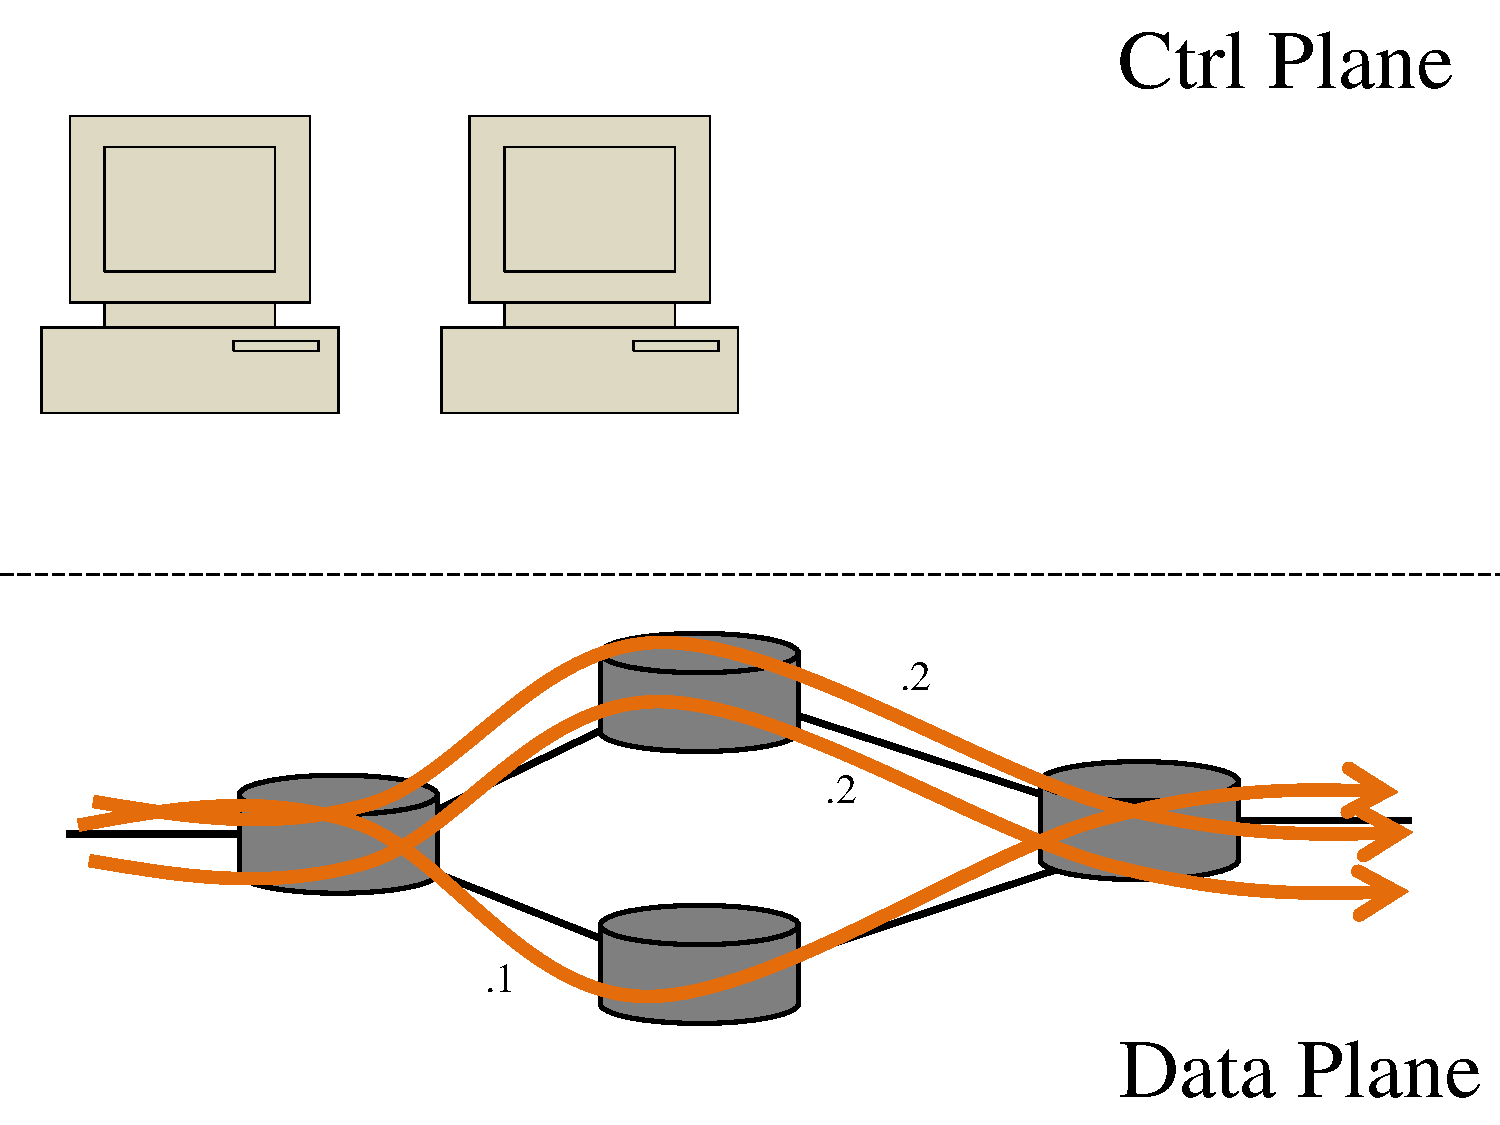
\includegraphics[width=0.35\columnwidth]{loadbal-before.pdf}~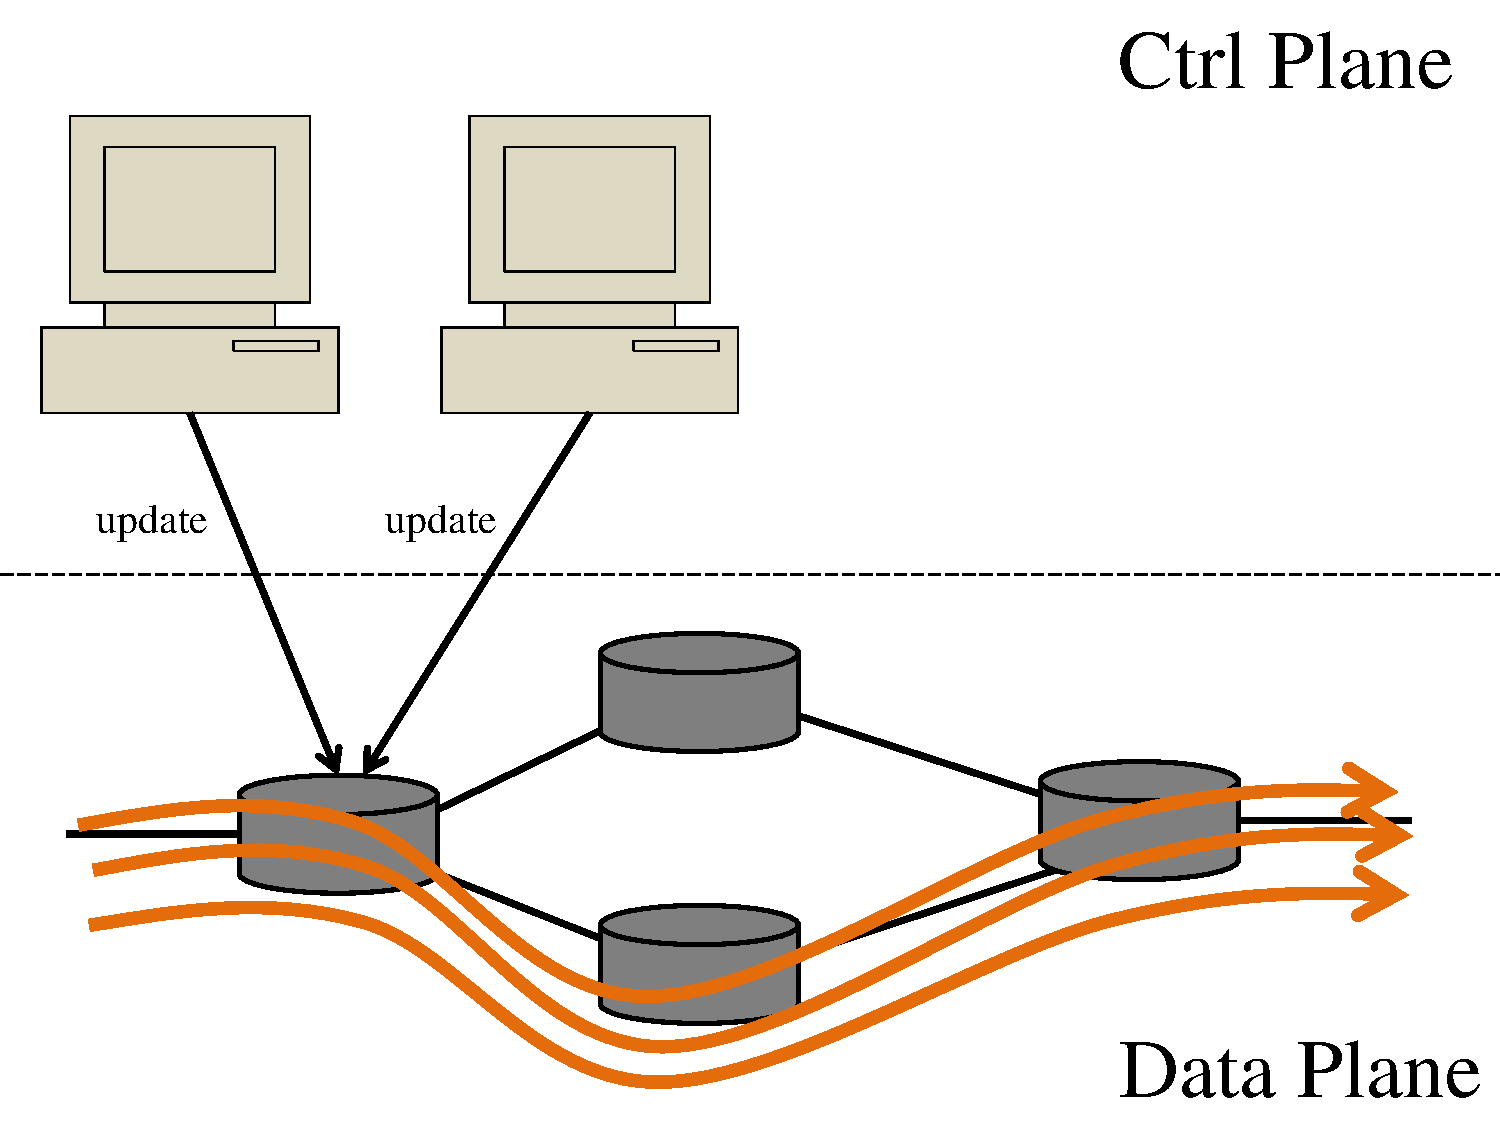
\includegraphics[width=0.35\columnwidth]{loadbal.pdf}~~
%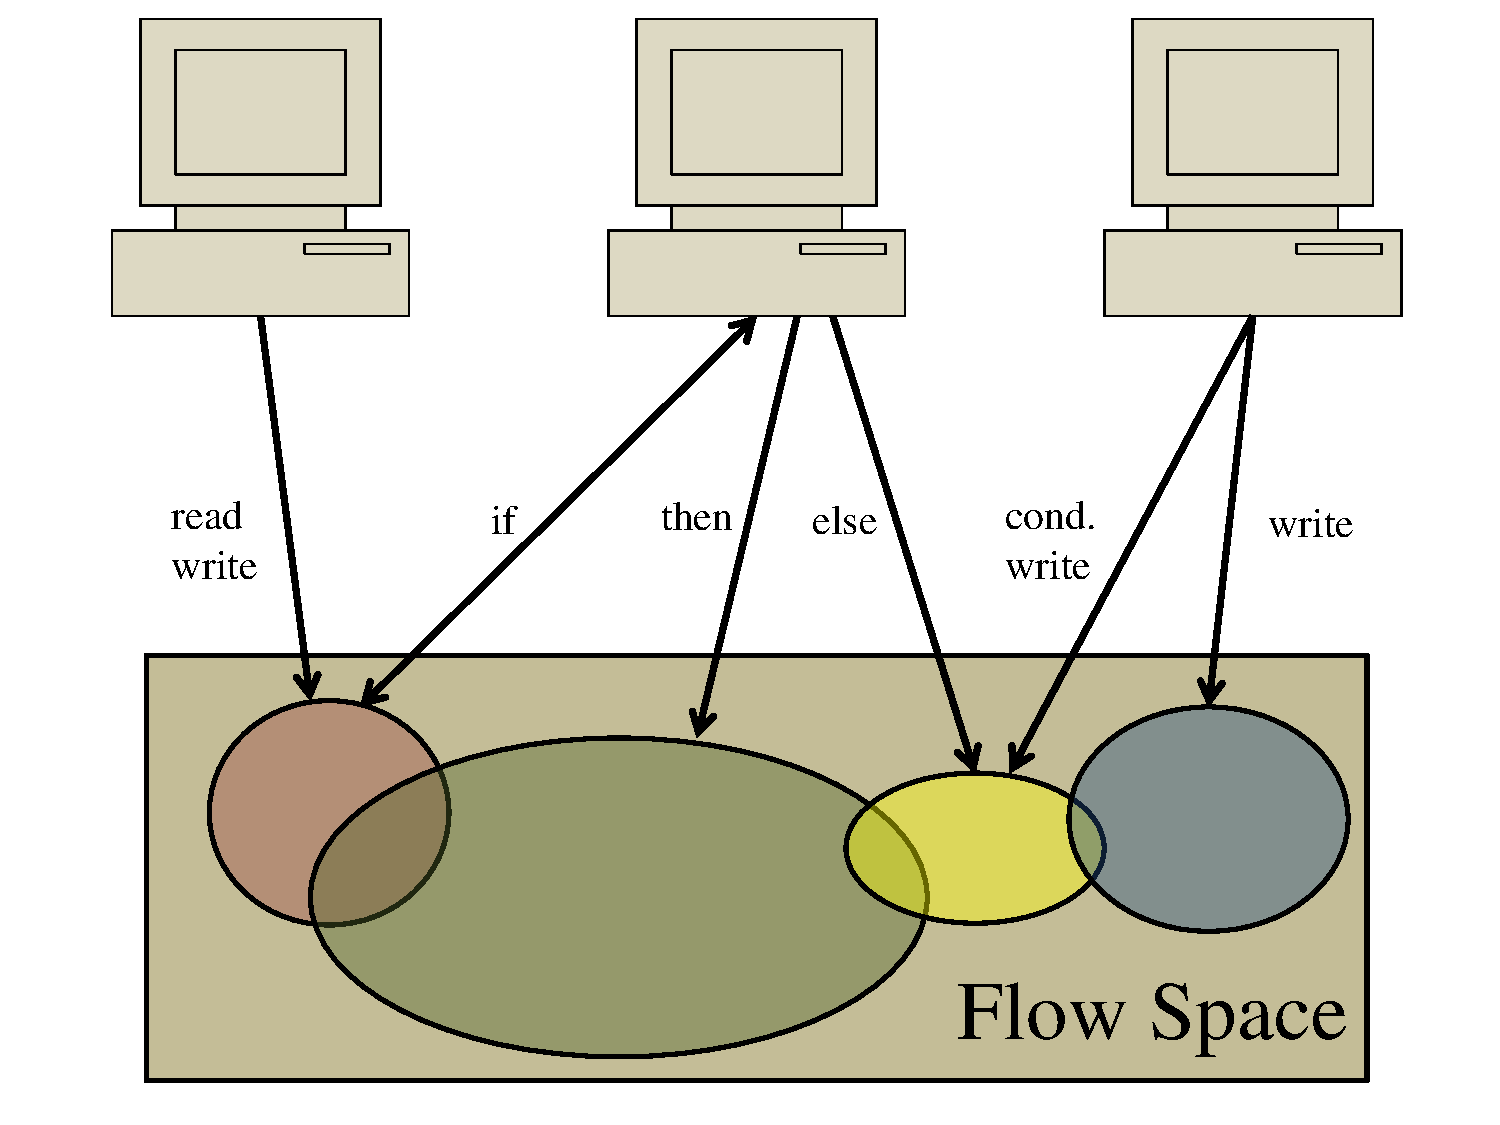
\includegraphics[width=0.8\columnwidth]{pic.pdf}\\
%\caption{\emph{Left:} Load-balancing gone wrong. \emph{Right:} Illustration of transactional abstraction which  allows
%controllers to modify switch configurations in complex ways,
%and
%depending on other flow spaces. Colors indicate different actions. \stefan{lets make two real transactions: one bundle and one 2 or 5 interactions?}}\label{fig:illu}
%\end{figure*}


\section{Limitations and Motivation}\label{sec:motivation}

% generic way for multiple distributed controllers to safely update switch configuration with no need of any control plane

At first sight, bundling \emph{FlowMod} commands with  the $\checko$
flag already provides a useful synchronization mechanism.
Indeed, its ``mini-transaction'' nature allows a controller
to install multiple flow entries in an atomic way.
%[[PK we did not say what reads and writes are...
%At first sight, the OpenFlow bundle feature seems to provide everything
%we need to implement our transactional interface \petr{did we say what we need already?}: the bundle
% defines a sequence of read and write operations
% on the switch state which is executed atomically.
%]]
However, as is,
%while the bundle can indeed be seen as a ``mini-transaction'',
bundling has important limitations, as we will argue in the following.
%\petr{unclear what "reads and writes" are here, not discussed before. How openflow can be used to implement reads and writes?}

First, %if employed without any additional features,
except for some limited constraint types (such as
overlapping flow spaces or insufficient free space),
a bundle does not provide any means to modify the switch configuration
based on application-specific conditions, which depend on the
current configuration,
However, as we will argue, a support for more generic conditions under which configuration
updates
should or should not take place, is often desirable.
%
%But also bundling FlowMod commands with the check overlap feature ($\checko$)
%comes with limitations: while it is possible
% to \emph{abort} a bundle depending on certain conditions
% in the \emph{overlapping
% flow spaces}, oftentimes it is desirable to be able
% to define more general conditions and notions of conflicts
% under which an atomic update should not take effect.
% \liron{replaced transaction in the last sentence with " atomic update"}
%
Second, sometimes it is desirable to react to conflicts in smarter ways than
by simply aborting an operation, e.g., by supporting \emph{conditional modifications}.
Let us consider two examples.

%\begin{enumerate}
\vspace{1mm}
\noindent \textbf{Example~1: Handling complex dependencies.} Let us consider two controllers
in charge
of \emph{load-balancing}, see Figure~\ref{fig:CAS-example}
for a simplistic example with two links.
In such a scenario, seemingly independent actions, defined over
completely independent logical flow spaces (say, two different
TCP micro-flows),
%originated in disjoint ranges of IP addresses),
may actually be dependent: the flows share the underlying physical network.
Accordingly, if multiple controllers concurrently and independently
update forwarding rules according to a na\"ive load-balancing algorithm \`{a} la Algorithm~\ref{alg:naive-lb},
they may involuntarily
unbalance the flow allocation.
Simple flow space overlap checks cannot be used to detect
such conflicts.
Note that, assuming that all these flows are
completely independent, bundling and $\checko$ features do not really
help here.

%Consider the example in the left part of Figure~\ref{fig:CAS-example}. Two controllers,
%$1$ and $2$ read the configuration, try to add two more flows to a switch
%with two outgoing links, balancing the load.
%Imagine that each of the controllers reads the switch configuration and
%learns that currently one flow is forwarded to the left link and two
%flows are forwarded to the right link.
%Without synchronization, the two controllers naturally choose to
%install their flows on the left link, which results in an undesirable
%unbalanced state.

{\small
\begin{algorithm}[t]
    \caption{$\textit{Na\"ive Flow Balancing}$}
    \label{alg:naive-lb}
\begin{algorithmic}[1]

    \Require \emph{new\_flows}: flow entries of the new flows,
    \emph{ports}: a list of switch output ports,
    \State $\textit{policy} \gets \textbf{read\_config}$
    \State $\textit{update\_cmds} \gets \textsc{lb\_update}(policy)$ %(new\_flows, ports, policy)$
    \State $\textbf{send}\{\textit{update\_cmds}\}$
%    \State $\textbf{execute-atomic}\{update\_cmds\}$
    \Statex

    \Statex \emph{\bf Function} $\textsc{lb\_update}(\textit{policy})$ % (new\_flows, ports, policy)}$

	\State $\textit{flows\_per\_port} \gets [0, 0, \ldots, 0]$
	\ForAll {$\textit{entry} \in \textit{policy}$}
	    \State $\textit{port} \gets \textit{entry.output\_port}$
	    \State $\textit{flows\_per\_port}[\textit{port}]++$
	\EndFor
	\State $\textit{new\_flow\_mod\_cmds} \gets \{\}$
	\For {$\textit{entry} \in \textit{new\_flows}$}
	    \State $\textit{port} \gets \arg\min_{p\in \textit{ports}} \textit{flows\_per\_port}[p]$
	    \State $\textit{entry.output\_port} \gets \textit{port}$
	    \State $\textit{flows\_per\_port}[\textit{port}]++$
	    \State $\textit{cmd} \gets \textit{FlowMod}(add,f)$
	    \State $\textit{new\_flow\_mod\_cmds}.\textit{add}(\textit{cmd})$
	\EndFor
	\Return $\textit{new\_flow\_mod\_cmds}$
  %  \State \emph{\bf EndFunction}
\end{algorithmic}
\end{algorithm}
}

%\petr{postpone the explanation of the right part of the figure until we come to CAS?}

\vspace{1mm}
\noindent\textbf{Example~2: Supporting modifications.}
Consider the arguably very basic problem of \emph{modifying} previously installed forwarding rules
in a consistent manner.
In principle, a bundle allows to conditionally add new rules or remove
old rules, and, using the flow space overlap
check feature $\checko$, to abort the transaction if potentially conflicting
rules were already there. However, it is not obvious how
to use the bundle to
modify \emph{existing} rules, especially if the modification depends on
specific conditions.
In other words, the bundle and overlap check only help
for the \emph{conditional creation} of rules, not their \emph{modification}.

\vspace{2mm}
\noindent\textbf{Our Approach.}
This paper proposes mechanisms to solve these two examples,
by using a minimal
``meta-configuration'' space. That is, controllers store information
on contention and conflicts between
concurrently installed policy updates on the switch. Controllers can read and modify
this meta-data by applying synchronization primitives.
In the following section, we
describe how this space can be organized and consistently maintained
by multiple controllers despite of concurrency and conflicts.

We will later come back to these examples, and show that Algorithm~\ref{alg:naive-lb}
can actually be used without any modifications within our framework.
Consistent load-balancing can also be achieved using our atomic Compare-and-Set instruction based on policy ids (pids),
see Figure~\ref{fig:CAS-example} (\emph{right}).

\begin{figure}[t]
\centering
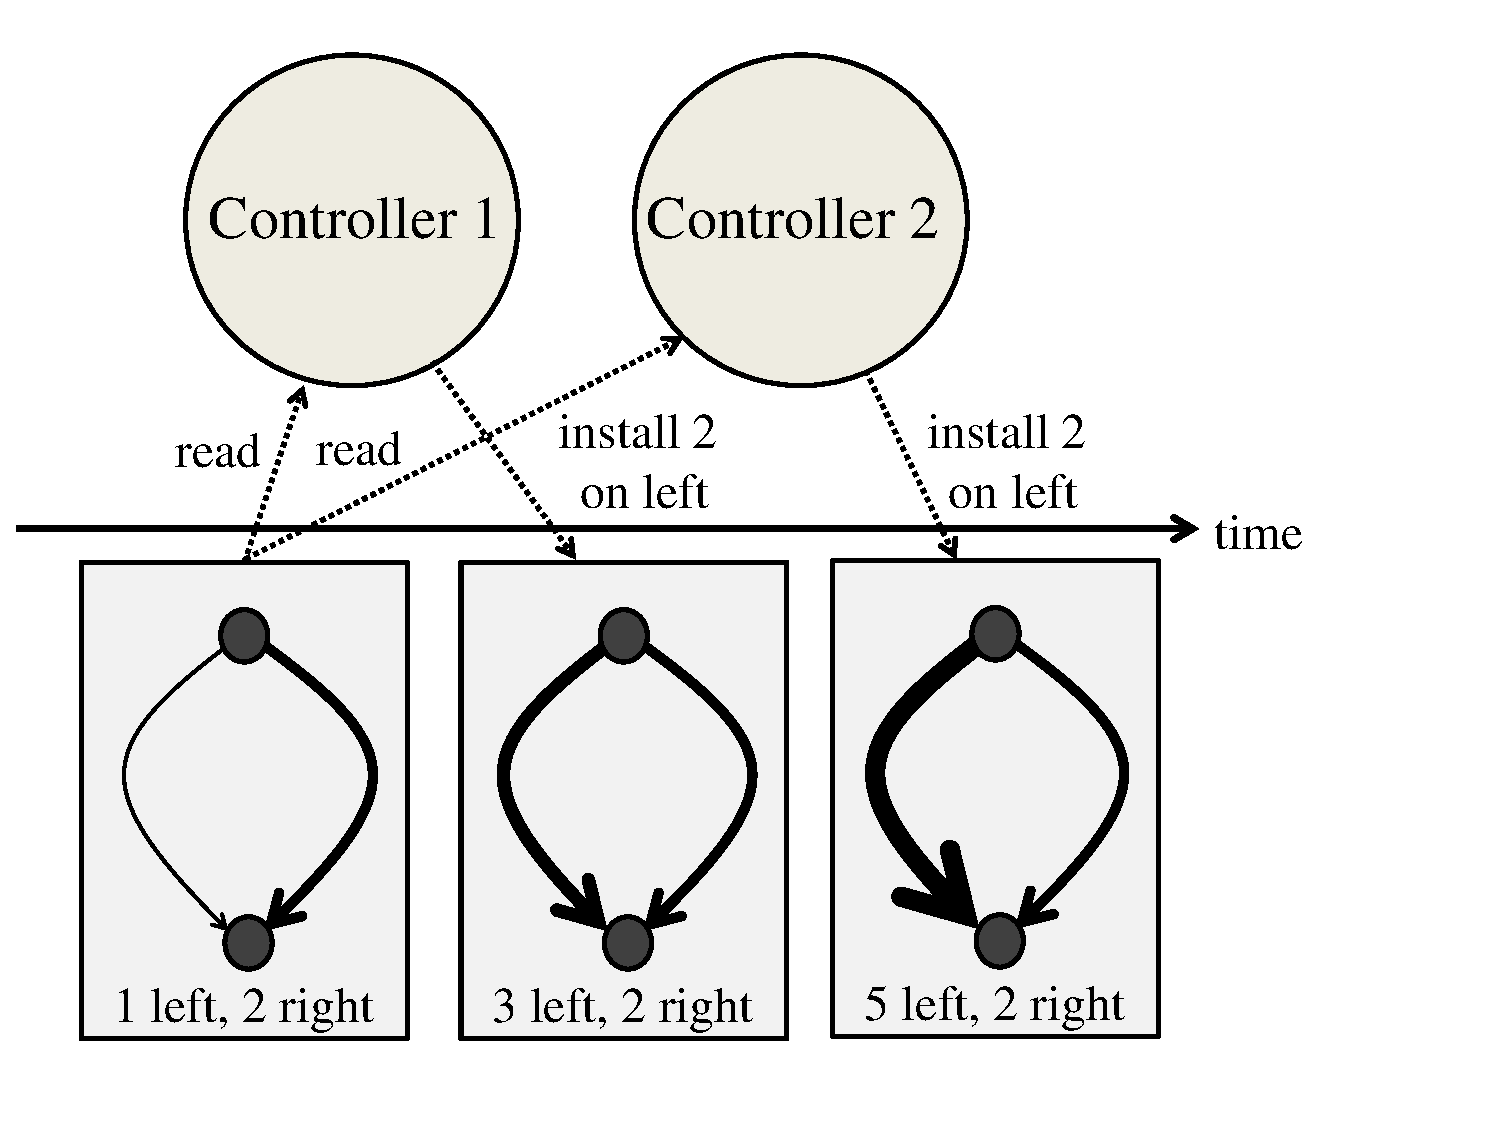
\includegraphics[width=.56\columnwidth]{loadbal-1.pdf}~\hspace{-.7cm}~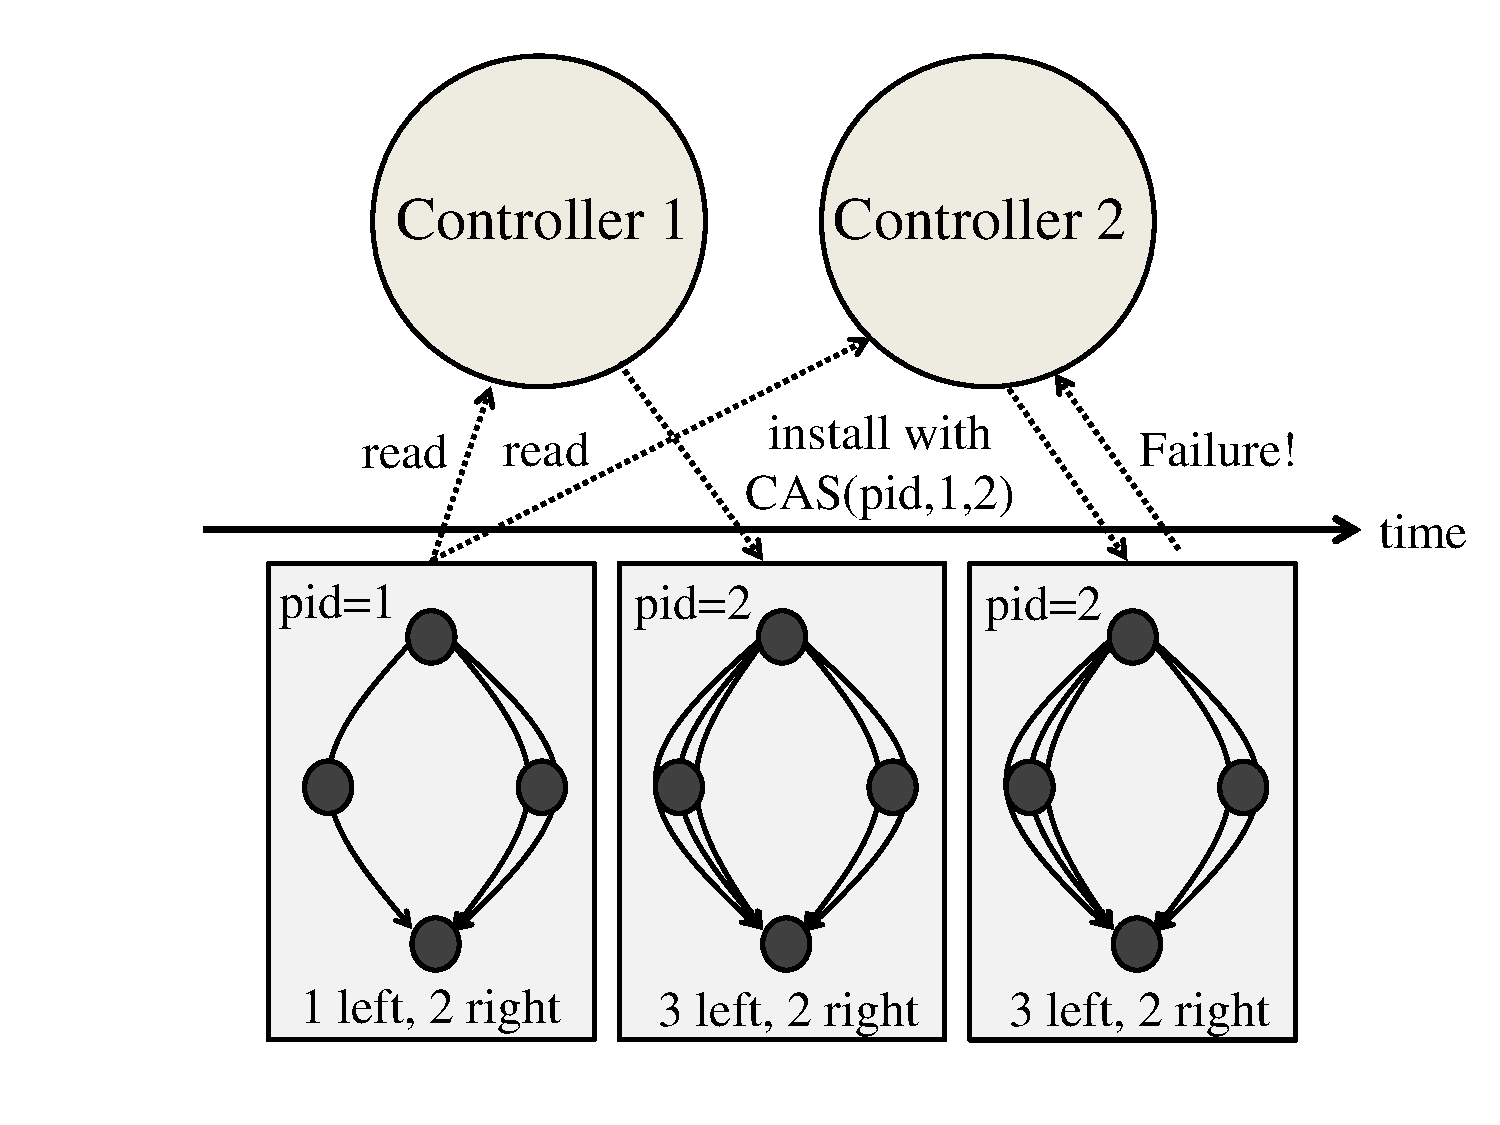
\includegraphics[width=.56\columnwidth]{loadbal-2.pdf}\\
\caption{\emph{Left:} Without synchronization, the two controllers naturally choose to
install their flows on the left link, which results in an undesirable
unbalanced state.
 \emph{Right:}
 With synchronization, i.e., by bundling the flow installation with a Compare-and-Set (CAS) primitive
 depending on the policy id (\emph{pid}), this problem is avoided.}\label{fig:CAS-example}
\end{figure}

%[[PK not really discussed?
%As we will see, we do not even need the bundle feature
%to implement the powerful synchronization objects of our transactional interface.
%However, the bundle feature can still be useful in the context of
%consistent policy updates.

%At first sight, a bundle seems to be a powerful concept
%for the implementation of a transactional interface. However,
%while the  bundle can indeed be seen as a ``mini-transaction'',
%in itself it is not very useful. In fact, as we will discuss
%in more detail in the next section, we will not make
%use of the bundle in the implementation of our synchronization
%objects, but will employ it for our case study
%of consistent policy updates.%
%
%Before presenting our transactional interface and implementation,
%let us first discuss the limitations of the OpenFlow features discussed above.

%\section{The Container Object}\label{sec:vision}

\section{Synchronization Abstractions}\label{sec:main}

We now describe how our  meta-configuration space at
an OpenFlow switch can be implemented and manipulated using our
synchronization framework.

\vspace{1mm}
\noindent\textbf{Configuration space.}
%
We distinguish two parts of the configuration space of a switch:
the ``normal'' configuration which determines the network policy and
is used to process the data plane traffic (e.g., forwarding rules),
and the \emph{meta-configuration} that contains information used by the
controllers to synchronize their actions.
Flow entries in the meta-configuration can be referred to as shared
memory locations, provided a total addressing scheme.

The meta-configuration is implemented as a set of flow entries
designed in a way that it does not affect the processing of data plane
traffic. One way to achieve this is to set a low priority to
the meta flow entries and ensure that the regular flow entries
maintain higher priority levels.
Alternatively, we could leverage the possibility to maintain multiple
flow tables at an OpenFlow switch, and use a separate flow table for
the meta-configuration,  making sure that the
\emph{pipelining} mechanism will never involve this
flow table.



%\petr{How to make sure that traffic is not affected by the ``meta'' part?}
\vspace{1mm}
\noindent\textbf{Synchronization.}
 %
Our framework provides the controllers with the ability to execute
sequences of \emph{operations} on the
switch configuration in an \emph{atomic} (transactional) or \emph{non-atomic} mode.
In the atomic mode, either \emph{all} operations in the sequence, henceforth simply
called \emph{transaction},
should be executed, or none (the transaction is rejected).
In the non-atomic mode, no atomicity guarantees are provided.
An operation here can be a regular FlowMod command or a synchronization
primitive, which, as we
show below, translates into a sequence of FlowMod commands operating on the
switch meta-configuration.

We propose the following constructs
%$\textbf{bundle}\{\;\ldots\;\}\rightarrow res$ to refer to represent a
$\exec\{op_1,\;\ldots\;op_k\}$ and $\execatomic\{op_1,\;\ldots\;op_k\}$
which execute a sequence of commands $op_1,\ldots,op_k$ in
a regular and atomic way, respectively.
The construct returns $\ack$ if the sequence of operations is performed and all commands are performed successfully, and
$\error(\xid,\ecode)$ received from the switch otherwise, providing
the identifier of the first command in the sequence that failed
together with the corresponding error code.
%Again, the bundle always returns a binary result: \emph{error} ($\bot$) or \emph{success} ($\top$).
%\petr{Should also provide the reason why the bundle has failed?}



\hide{
Given this motivation, we now present a more powerful transactional interface.
At a high level, we aim to export a
transactional interface which allows each controller $i\in[N]$ ($N\geq
2$) to perform multiple
operations on the configuration of an OpenFlow switch as an atomic
\emph{transaction}, inspired by the transactional-memory paradigm~\cite{stm-st95,tm-book}. A transaction may \emph{commit}, in
which case it appears as executed sequentially, or \emph{abort}, in
which none of its operations takes effect.
}

\vspace{1mm}
\noindent\textbf{Synchronization primitives.}
%
\hide{

Our approach is based on the distributed management of \emph{identifiers (IDs)} \petr{unclear what "identifiers" mean here}. In particular,
we introduce two new synchronization objects (and describe their implementation in standard OpenFlow),
which allow controllers to coordinate
themselves based on these identifiers.

As we will see, in the OpenFlow implementation of our mechanism,
in addition to the ``normal'' configuration stored at the switch
(e.g., forwarding rules according to network policies),
controllers will maintain additional information
in the switch configuration: this information is used by the
controllers to synchronize.
\petr{"As we will see,..." - looks funny compared with "As we will see ..." at the end of Sec 2}
\subsection{Synchronization Objects}\label{sec:t-if}
}
%
We focus first on the consistent use of  \emph{policy identifiers},
an important notion in consistent policy updates~\cite{network-update,stn}.
Intuitively, a controller should
equip each to-be-installed policy with a distinct
identifier,
%[[PK do not want to say ``unique'': we also need to motivate claimer-id]]
and the installation should succeed only if the identifier of the
currently installed policy has not changed since the last time the
controller read it.

Therefore, we provide the following transactional operations.
A $\textit{write}(\addr,k)$ operation sets the content at memory location
$\addr$ to $k$.
%
%For  example, the offset $\addr$ may correspond to the policy identifier (\emph{pid}),
%  but our approach is more general.
%
A $\textit{\compare}(\addr,k)$ operation \emph{aborts} the transaction
if and only if the content at
$\addr$ is \emph{not} $k$.
Intuitively, by combining compare and write with a set of regular
FlowMod commands in a transaction we can make sure that the
configuration is changed and the current policy identifier is updated
only if the check operation \emph{succeeds} (does not abort).

To make sure that policy identifiers do not grow without bound~\cite{stn}, we
also provide an \emph{id-claimer} object.
The object implements a weak type
of locking by allowing a controller to claim a \emph{resource identifier} in a
given set, release an identifier,  and check if a given identifier
is currently claimed by any controller.
%While In theory one can use the memory abstraction to implement the resource claimer,
%however we found it far more simple and efficient to consider the resource claimer as base object.
%
More precisely, the id-claimer object exports three operations \emph{claim},
\emph{unclaim} and \emph{\claimcheck} with the following sequential
semantics:
%The container synchronization object introduced in this paper
%is essentially a transactional memory abstraction which can be implemented
%in standard OpenFlow switches.
%Before presenting the technical details in the next section,%
%we give a brief overview.

%The postulated container object can store an arbitrary number of \emph{items}.
%As we will see, these items correspond to flow entries on the OpenFlow switch.
%The same item may even exist multiple times in the container (i.e., the container
%is a multi-set).
%The container
%provides two main functions:
\begin{itemize}
\item With $\textit{claim}(k)$,
%  $k\in\Nat$,
a controller %$i\in[N]$
\emph{claims}  identifier $k$.

\item With $\textit{unclaim}(k)$, %$k\in\Nat$,
the controller %$i\in[N]$
  \emph{unclaims} identifier $k$.
An identifier $k$ is called \emph{claimed} at a given point of an
execution if there is a controller that has performed $\textit{claim}(k)$
but has not yet performed  $\textit{unclaim}(k)$.

\item If $k$ is currently claimed by any controller,
$\textit{\claimcheck}(k)$ %, $k\in\Nat$,
aborts the current transaction.
%returns $\textit{true}$ if and
%  only if $k$ is not currently claimed by any controller; if
%  $\textit{false}$ is returned, we say that the check operation
%  \emph{fails} (which causes an abort of the transaction invoking it).

\end{itemize}

%As we will see, the bundle feature is not required to implement these semantics.
%Also note that memory read operations correspond to reading the switch
%configuration, and are simple as they do not affect the execution of the transaction
%(unlike the $\textit{\compare}$ operation). \petr{read operations "do not affect the execution of the transaction" appears strange, given that a transaction, if committed, "appears to execute sequentially". Something seems wrong here...}


\begin{comment}
\subsection{Interface}\label{sec:t-if}

\liron{this subsection doesn't flow well for me}

We assume that transactions may comprise operations on the flow table
of an SDN switch. Our transactional abstraction exports the
$\textbf{bundle}\{\;\ldots\;\}$ construct
containing a sequence of transactional
operations and may \emph{commit} and return responses to all its operations
or \emph{abort} (so that none of its operation takes effect).
We guarantee that in every execution, all committed
transactions constitute a \emph{legal} sequential
order~\cite{Pap79-serial}, i.e., every transaction appears as executed
sequentially. On the progress side, we ensure that a
transaction $T$ is only allowed to abort if either another
transaction updated a flow table entry read by $T$
or if one of $T$'s operations (\textit{check} or CAS) fails.
We employ the \emph{deferred-update} semantics:
no transaction can affect other transactions before it commits.
In particular, if a controller crashes before committing its
transactions, no future transaction can be affected.
%Note that
%, assuming such a transactional memory,
%a $\emph{contains}(x)$ operation can be implemented as a transaction
%composed of $\textit{cond-add}(x)$ followed by $\textit{cond-delete}(x)$.
%A \emph{set} abstraction is a special instance of a multi-set that is
%only modified with \textit{cond-add} and \textit{cond-delete}
%operations (this way the set only contains at most one copy of a given
%item).

\end{comment}

\vspace{1mm}
\noindent\textbf{Implementation.} %\label{sec:t-impl}
%
We now describe how to implement our transactional
abstractions using standard OpenFlow features.
Essentially, we translate each of the transactional operations into a
sequence of FlowMod commands.

The implementation of $\exec\{op_1,\ldots,op_k\}$ and
$\execatomic\{op_1,\ldots,op_k\}$ constructs
invoked by a control application is simple.
First we translate  $op_1,\ldots,op_k$ into a sequence of FlowMod
commands. If $op_i$ is already a FlowMod command, the translation is
trivial. If $op_i$ is a synchronization primitive, we employ
Algorithm~\ref{alg:claim} for $\textit{claim}$,
Algorithm~\ref{alg:check} for $\textit{checkclaim}$,
Algorithm~\ref{alg:unclaim}
for $\textit{unclaim}$,
Algorithm~\ref{alg:write} for $\textit{write}$ and
Algorithm~\ref{alg:compare} for $\textit{compare}$.

To implement  $\exec\{op_1,\ldots,op_k\}$, we simply send the commands in
the resulting sequence, one by one, to the switch.
%
To implement  $\execatomic\{op_1,\ldots,op_k\}$, we
additionally create a bundle, wrap each of the resulting commands in a
bundle message with the corresponding bundle identifier, and complete it
with a bundle commit message.
Then we wait until the
corresponding responses are received.
If an error message is return,
it is forwarded to the control application,
otherwise it is $\ack$ed.

We now describe Algorithms~\ref{alg:claim}-\ref{alg:compare} in more
detail.
Each of the operations generates one or two FlowMod commands.
The \textit{match} part in these commands specifies only the $64$bit meta-data
field in the header space, leaving the remaining fields at default
values.
In defining the value and the mask,
% of the math part,
we
use the notation $a\concat b$ to represent a concatenation of two
$32$bit integers $a$ and $b$: $a\concat b := (a<<32)+b$.
We also write \texttt{1$\ldots$1} for  a $32$bit
string of $1$'s used in a mask.
%
The action part in these commands is defined as an integer, which in
practice can be implemented by a \emph{set meta-data} instruction where the written value is that integer.


\hide{
%[[PK too lengthy, partially said before
To simplify the presentation we set the FlowMod command field values with integers, according to the following guidelines:
\begin{itemize}

\item {\bf  Flag:} we often use the $\checko$ optional flag value to make the command execution dependent on switch state. In other cases, when the flag value remains zero, we omit the assignment.

\item {\bf  Match:} we consider the match part of an entry to be a ternary string of bounded length, represented by binary strings (integers) named value and mask. In general, the match can be applied to any set of supported packet header fields. In our implementation, the $64$bit meta-data field alone is sufficient. We sometimes use the concatenation of two $32$bit integers, denoted by $a\concat b$, to form one match value or mask, where $a\concat b := (a<<32)+b$.

\item {\bf Action:} we consider the action part of an entry to be an integer, which in practice can be implemented by a \emph{set meta-data} instruction where the written value is that integer.

\end{itemize}

In addition we use "op" as shortened form to a field that indicates whether the command should $\add$ or $\dele$ the specified flow entry. This corresponds to the FlowMod field named "command" which can receive values \textt{ofpfc\_add} and \texttt{ofpfc\_delete}.
%]]
}

\vspace{1mm}
\noindent\textbf{The id-claimer.}
%
In Algorithms \ref{alg:claim}-\ref{alg:unclaim},
the match part of the constructed commands represents a concatenation
of two claimed identifiers.
In addition, every controller uses a unique mask part of the match
defined as a distinct $32$bit controller identifier concatenated with
\texttt{1$\ldots$1}.
This allows multiple controllers to claim the same identifier without
overriding existing flow entries.
%
For example, for any two resource identifiers $x_1$ and $x_2$ and controller identifiers $c_1\neq c_2$,
the match patterns $m_1=(x_1\concat x_1, c_1\concat \texttt{1$\ldots$1})$ and $ m_2=(x_2\concat x_2, c_2\concat \texttt{1$\ldots$1})$ are distinct,
even if $x_1=x_2$.
Therefore, they can both be used to claim and unclaim identifiers without affecting each other.

In order to check if an identifier is claimed, a controller tries to add
a new entry setting the flag \texttt{\checko}, and using a different
action ($2$ instead of $1$),
thereby inflicting a failure in case an entry with overlapping match value exists.
If the check succeeds, we delete the entry.
Considering $m_1$ and $m_2$ from the example above,
with respective actions $a_1=1$ and $a_2=2$,  they overlap
with different actions iff $x_1=x_2$. Therefore, if $m_1$ is used in the \claimcheck after $m_2$ was used in the claim operation,
a conflict is detected iff $x_1=x_2$, as desired.

Note that in order to save space, when checking for claims, also the deletion of the added tester flow entry is included,
which however has no effect on claims and checks of other controllers; hence, the deletion command does not
have to be sent as part of a bundle. Therefore, the \texttt{\claimcheck} operation is atomic by nature,
similar to the \texttt{claim} and \texttt{unclaim} operations, and is
implemented as essentially one command.

By employing the \textbf{read-config} command, we may easily implement
an additional operation that returns all currently claimed ids: it is
sufficient to go over the rules matching every controller identifier.

%A container contains items: they represent the flow table entries (i.e., a match-action rules, plus e.g., counters belonging to the rule).
%Items can be added and removed atomically and in bundles (e.g., to update the switch with
%a new policy). Recall that we want to add items only if they do not exist
%yet; otherwise the transaction should abort without taking effect.
%And similarly for removes: transactions should not take effect if the corresponding
%update contains rules which currently do not exist at the switch.

{\small

\begin{algorithm}[t]
    \caption{$\textit{claim}(x)$}
    \label{alg:claim}
    \begin{algorithmic}[1]
    \Require \emph{self} as the calling controller id.
%    \Ensure
    		\State $\textit{value} \gets x\concat x$
    		\State $\textit{mask} \gets \textit{self}\concat \texttt{1$\ldots$1}$
	    	\State $\textit{match} \gets (\textit{value},\textit{mask})$
    		%\State $cookie \gets x\concat self$
    		\State $\textit{action} \gets 1$
    		\State $\textit{flag} \gets 0$
    		\State $\textit{cmd}\gets \textit{FlowMod}(match, op = \add, \textit{flag}, \textit{action}) $
			\Return $\textit{cmd}$
    \end{algorithmic}
\end{algorithm}

\begin{algorithm}[t]
    \caption{$\textit{\claimcheck}(x)$}
    \label{alg:check}
    \begin{algorithmic}[1]
    \Require \emph{self} as the calling controller identifier.
%    \Ensure
    		\State $\textit{value} \gets x\concat x$
    		\State $\textit{mask} \gets self\concat \texttt{1$\ldots$1}$
    		\State $\textit{match} \gets (value,mask)$
    		%\State $cookie \gets x\concat self$
    		\State $\textit{action} \gets 2$
    		\State $\textit{flag} \gets \texttt{ofpff\_\checko}$
    		\State $\textit{cmd1}\gets \textit{FlowMod}(\textit{match}, op = \add, \textit{flag}, \textit{action}) $
    		\State $\textit{cmd2}\gets \textit{FlowMod}(\textit{match}, op = \dele) $
			\Return $\textit{cmd1}$,$\textit{cmd2}$
    \end{algorithmic}
\end{algorithm}

\begin{algorithm}[t]
    \caption{$\textit{unclaim}(x)$}
    \label{alg:unclaim}
    \begin{algorithmic}[1]
    \Require \emph{self} as the calling controller id.
%    \Ensure
    		\State $\textit{value} \gets x\concat x$
    		\State $\textit{mask} \gets self\concat \texttt{1$\ldots$1}$
    		%\State $cookie \gets x\concat self$
    		\State $\textit{match} \gets (\textit{value},\textit{mask})$
    		\State $\textit{cmd}\gets \textit{FlowMod}(\textit{match}, op=\dele) $
    	
			
			\Return $cmd$
    \end{algorithmic}
\end{algorithm}
}

\vspace{1mm}
\noindent\textbf{Write and compare.}
The memory \memwrite and \compare
 operations can be implemented using similar techniques.
 As can be seen in Algorithms \ref{alg:write}-\ref{alg:compare},
  the match part of the added flow entry is used as the memory address and the action as
  the written value. Values written to the same address will replace one another,
following the command definition to replace the old flow entry with a new one in case they
share the same match parts.

In order to check if a value is written at a given address,
we try to add it the same way as in the \memwrite operation,
but we also set the \texttt{\checko} flag. If the value is not there,
our action differs from the action of the existing entry,
thereby inflicting a failure.
In case the value is there, our flow entry replaces the existing flow entry
with an identical one.

%HERE: we can read state by reading flow monitor => read configuraiton abstraction => state of claimer ID objects list of all claimed identifiers

\begin{algorithm}[t]
    \caption{$\textit{write}(\addr,k)$}
    \label{alg:write}
    \begin{algorithmic}[1]
    %\Require  id $i$.
%    \Ensure
    		\State $value \gets \addr$
    		\State $mask \gets  \texttt{1$\ldots$1}. \texttt{1$\ldots$1}$
    		\State $match \gets (value,mask)$
    		%\State $cookie \gets x\concat self$
    		\State $action \gets k$
    		\State $flag \gets 0$
    		\State $cmd\gets \emph{FlowMod}(match, op = \add, flag, action) $
			\Return $cmd$
    \end{algorithmic}
\end{algorithm}

\begin{algorithm}[t]
    \caption{$\textit{\compare}(\addr,k)$}
    \label{alg:compare}
    \begin{algorithmic}[1]
    %\Require  id $i$.
%    \Ensure
    		\State $value \gets \addr$
    		\State $mask \gets  \texttt{1$\ldots$1}.\texttt{1$\ldots$1}$
    		\State $match \gets (value,mask)$
    		%\State $cookie \gets x\concat self$
    		\State $action \gets k$
    		\State $flag \gets \texttt{ofpff\_\checko}$
    		\State $cmd\gets \emph{FlowMod}(match, op = \add, flag, action) $
			\Return $cmd$
    \end{algorithmic}
\end{algorithm}




\section{Applications}\label{sec:apps}

Our synchronization mechanisms can be useful in many situations.
For example, it can be used to implement the fundamental
\emph{Compare-and-Set} (CAS) operation. % on the policy identifier.
When executed within a
transaction, a $\cas(\addr,\textit{old},\textit{new})$ operation 
on a memory location $\addr$
checks if the content of $\addr$ is $\textit{old}$ and if so,
replaces it with $\textit{new}$ %and returns $\true$ 
(the CAS \emph{succeeds}), otherwise it 
%returns $\false$ 
causes an abort of the invoking transaction
(the CAS \emph{fails}).
It is straightforward to implement the CAS operation by executing
$\textit{\compare}(\addr, old)$ followed by $\textit{\memwrite}(\addr,
new)$ within the {\execatomic} construct.

%[[PK said it in the text
\hide{
As can be seen Algorithm \ref{alg:cas}, CAS is implemented by two commands. These commands should be sent as part of the same bundle

\begin{algorithm}[t]
    \caption{$\textit{\cas}(\addr, old,new)$}
    \label{alg:cas}
    \begin{algorithmic}[1]
    %\Require  id $i$.
%    \Ensure

    		\State $cmd1\gets \textsc{\compare}(\addr, old) $
    		\State $cmd2\gets \textsc{\memwrite}(\addr, new) $
			\Return $cmd1,cmd2$
    \end{algorithmic}
\end{algorithm}
}
%]]

CAS can be used to solve the fundamental
problem of fault-tolerant \emph{consensus}~\cite{FLP85}
\hide{%[[PK, feels like we do not really need this level of detail here
 in which the controllers
need to agree on one of their private inputs, despite failures of an
arbitrary number of controllers.
Indeed, each controller simply performs, within a transaction, a CAS operation to replace the default value
in a memory location at the meta-configuration of a data plane switch.
If the transaction commits, the controller considers itself
the \emph{winner} and decides on its input,
if it aborts (the controller fails in the CAS), it remains to read the
memory to get the input of the winner and decide on it.
}
and allows us
to implement any generic replicated state machine~\cite{Her91}
in the control plane,  in the \emph{wait-free} manner, i.e., tolerating
asynchrony and failure of any number of controllers.
As such, CAS can also be used to implement STN~\cite{stn},
by providing the postulated \emph{read-modify-write} object.

%which will be instrumental in the
%next section.

%Moreover, given the CAS, we can also implement more complex operations,
%for example the replicated state machine postulated in STN~\cite{stn}:
%in order to choose tags in a consistent manner, CAS needs to be enhanced%
%with a notion of tags.

%\petr{when talking about replicated state machines, we should make it clear that we that we talk about replication among controllers.}

%\petr{"more complex operations": more complex than what?}

%\petr{the discussion of CAS in STN is confusing, given that we never described STN.}

Our mechanism can also be used as a generic template to
implement concurrent policy compositions of a user-specific
$\textsc{\ufunc}()$ function~\cite{stn}.
This way, for example, by choosing our load-balancing
function $\textsc{lb\_update}$ (Example~1 in
Section~\ref{sec:motivation}), 
the pathological scenario described in 
Figure~\ref{fig:CAS-example} can be resolved.
% if we put
%the policy update in our transactional $\execatomic$ construct together
% with a \emph{Compare-and-Set} (CAS) operation on the policy identifier.

Let us first  consider a simple policy update protocol that
allows a set of  controllers to concurrently update switch policies, i.e., sets of
%[[PK policies have been defined in Background]]
effective flow entries, under the
condition that these rules can be \emph{composed} with the currently installed
policy.
Algorithm~\ref{alg:simple-update} uses the bundle feature to update
the switch configuration, where the configuration contains both the
policy and a meta-configuration memory address $\paddr$ that holds the \emph{policy identifier (pid)} .
In the algorithm, the controller first reads the currently installed
policy together with its {\pid},  applies the
$\textsc{\ufunc}()$ function to the current policy which results in a
set of update FlowMod commands and then tries to apply them
atomically together with a CAS operation on $\paddr$ replacing $\pid$
with $\pid+1$.
The latter ensures that if, concurrently, a new policy (with a different identifier) has been installed, the update
fails and takes no effect.
Algorithm~\ref{alg:simple-update} can therefore also be used
to render our na\"ive load-balancing Algorithm~\ref{alg:naive-lb}
consistent, without any modifications in the update function.

% \liron{the term composition doesn't make sense now with the new user update function... }

%\liron{we can explain how a normal controller code can be instrumented to use our paradigm}
%\petr{did not get the comment}

%[[PK clear from the algorithm?]]
% and use them in order to make sure that the new policy, with id
%$pid+1$, replaces the (what considered as) current policy, with id
%$pid$.
%Considering the policies identifiers, we send the policy update
%commands as part of a bundle that also tries to perform
%$CAS(pid,pid+1)$, thereby insuring that the commands are
%performed iff the current policy is still there and preventing other
%controllers to replace the new policy with another without observing it.

%\petr{what does it mean for an update function to be ``unsafe''?}

%For brevity, we omit explicitly putting the $\textbf{bundle}\{...\}$ construct
%around each of the transactional operation used in the algorithm.
%Indeed, since \textit{claim} and \textit{unclaim} operations cannot
%cause the corresponding transaction, we can assume that all
%``singleton'' (consisting of one operation only)  transactions
%containing such operations always commit. \liron{I think we can ommit this paragraph entirely - no need for bundle when it is not written}

{\small
\begin{algorithm}[t]
    \caption{Policy update with only CAS}
    \label{alg:simple-update}
    \begin{algorithmic}[1]
    \Require policy update function \textsc{\ufunc}, policy id address $\paddr$
    \Ensure installed policy is consistent with previous one
 		%\Do
 		\Repeat
 			\State $\pid,\textit{policy}\gets$ \textbf{read-config} %switch configuration}
 			\State $\textit{update\_cmds}\gets \textsc{\ufunc}(policy)$
 			\startTxn
	 			\State $CAS(\paddr,\pid,\pid+1)$,
	 			\State $\textit{update\_cmds}$ %conditioned on $metadata=my\_a$
	 			%\State update policy selector to $my\_a$
 			\endTxn
     		%\State $res \gets $ commit transaction
     	\Until{$\textit{res}=\ack$}
     	%\doWhile{$res=False$}
%   \vspace{3mm}
			\Return $\textit{res}$

    \end{algorithmic}
\end{algorithm}
}

%Note that in Algorithm~\ref{alg:simple-update}, policies identifiers
%grow without bound.
%However, as was observed in~\cite{stn}, the number of currently
%used identifiers can be made proportional to the number of concurrent
%controllers.
%
\hide{
It takes a set of rules $U$ (not yet a policy)and proceeds as follows: first, we seek to
 obtain a unique \emph{id}. FIXME: to be continued...
 \textbf{LS: I am not sure if I need to tell every step of the story or maybe it best to explain the main dif from the previous one similarly to what I just wrote next}.
}
%

%Algorithm~\ref{alg:update} uses our id-claimer abstraction
%to bound the number of policy identifiers.
%Claiming a policy id prevents another controller from using it with a
%different policy.
%A controller claims the current policy identifier, chooses a new id
%from a finite set of identifiers,
%and then checks that the new policy id is not claimed by another controller.
%Note that in Algorithm \ref{alg:update}, the meta-configuration is
%used to store $\textit{pid}$ and id-claimer.
%\petr{The description is not very clear.}

Algorithm~\ref{alg:update} is a more efficient alternative 
to Algorithm~\ref{alg:simple-update}. It uses our id-claimer abstraction
to bound the number of used policy identifiers.
Here, the controller first reads the current policy id and claims to prevent another controller from using it 
for a
different policy (Lines~\ref{update:read-config1}-\ref{update:read-config2}).
%Then it reads the configuration again in case the policy was changed just before claiming its id.
%Then considering other claims the controller chooses
Then the controller claims the first \emph{unused} id and computes the update commands to be executed (Line~\ref{update:compute}).
Finally, within an atomic transaction (\textbf{\execatomic}), it verifies whether the chosen policy id has not
been claimed and that
the policy has not been concurrently modified, and then updates the policy.
%[[PK added a note to the id-claimer description
%Note that in Algorithm \ref{alg:update}, the meta-configuration is
%used to store $\textit{pid}$ and id-claimer (the claims).


\hide{
We compute our new suggested policy by applying the update requests on
top of current policy, supporting any kind of requests and
policies. Then we make a transaction (using the bundle feature) to
atomically check that our policy id is not blocked by another controller, to change the current policy id to ours (an action that would fail if the current policy id is no longer what we are counting of) and to actually configure our new policy.

If one of the actions in the transaction fails we try again. There is no progress guaranty for each controller but there is one for the whole system - at least one of the controller will succeed in fulfilling its update requirements.
}

{\small
\begin{algorithm}[t]
    \caption{Advanced policy update}
    \label{alg:update}
    \begin{algorithmic}[1]
        \Require policy update function \textsc{\ufunc}, policy id address $\paddr$, id space $C$.
    \Ensure installed policy is consistent with previous one
 		%\Do
 		\Repeat
		 	\State $\pid,claims,policy\gets$ \textbf{read-config} \label{update:read-config1} %switch configuration
 			\State $\textbf{execute}\{claim(\pid)\}$
 			\State $\pid 2,\textit{claims},\textit{policy}\gets$ \textbf{read-config} \label{update:read-config2} %switch configuration
 			\If {$\pid\neq \pid 2$}
	 			\State $\textbf{execute} \{\textit{unclaim}(\pid)\}$
 				\State {\bf continue} (\textbf{restart} loop)
 			\EndIf
 			\State $\textit{my\_id}\gets$ choose a number from $C\setminus claims$
 			\State $\textit{update\_cmds}\gets \textsc{\ufunc}(policy)$ \label{update:compute}
 			\startTxn
 				\State $\claimcheck(my\_id)$,
	 			\State $CAS(\paddr, \pid,my\_id)$,
	 			\State $\textit{update\_cmds}$ %conditioned on $metadata=my\_a$
	 			%\State update policy selector to $my\_a$
 			\endTxn
	 		\State $\textbf{execute} \{\textit{unclaim}(\pid)\}$
     		%\State $res \gets $ commit transaction
     	\Until{$res=\ack$}
     	%\doWhile{$res=False$}
%   \vspace{3mm}
			\Return $\textit{res}$

    \end{algorithmic}
\end{algorithm}
}


%\noindent\textbf{One-Shot Update} FIXME: desribe how to implement one-shot update
%
%\noindent\textbf{STN}
%
%\textbf{TODO}
%

\begin{comment}
\section{In-Band Composition}\label{sec:compo}

We conclude our technical contribution by showing that sometimes,
powerful synchronization mechanisms can be implemented
in-band \emph{even without bundles}.
Concretely, we show that sometimes it is even possible
to automatically compose updates originating from different controllers,
in-band and just using OpenFlow.

To illustrate this point, we consider a simple example
with two controllers concurrently issuing updates to a single
given switch.

FIXME: Explain, maybe even with an example?

\begin{figure}[t]
\centering
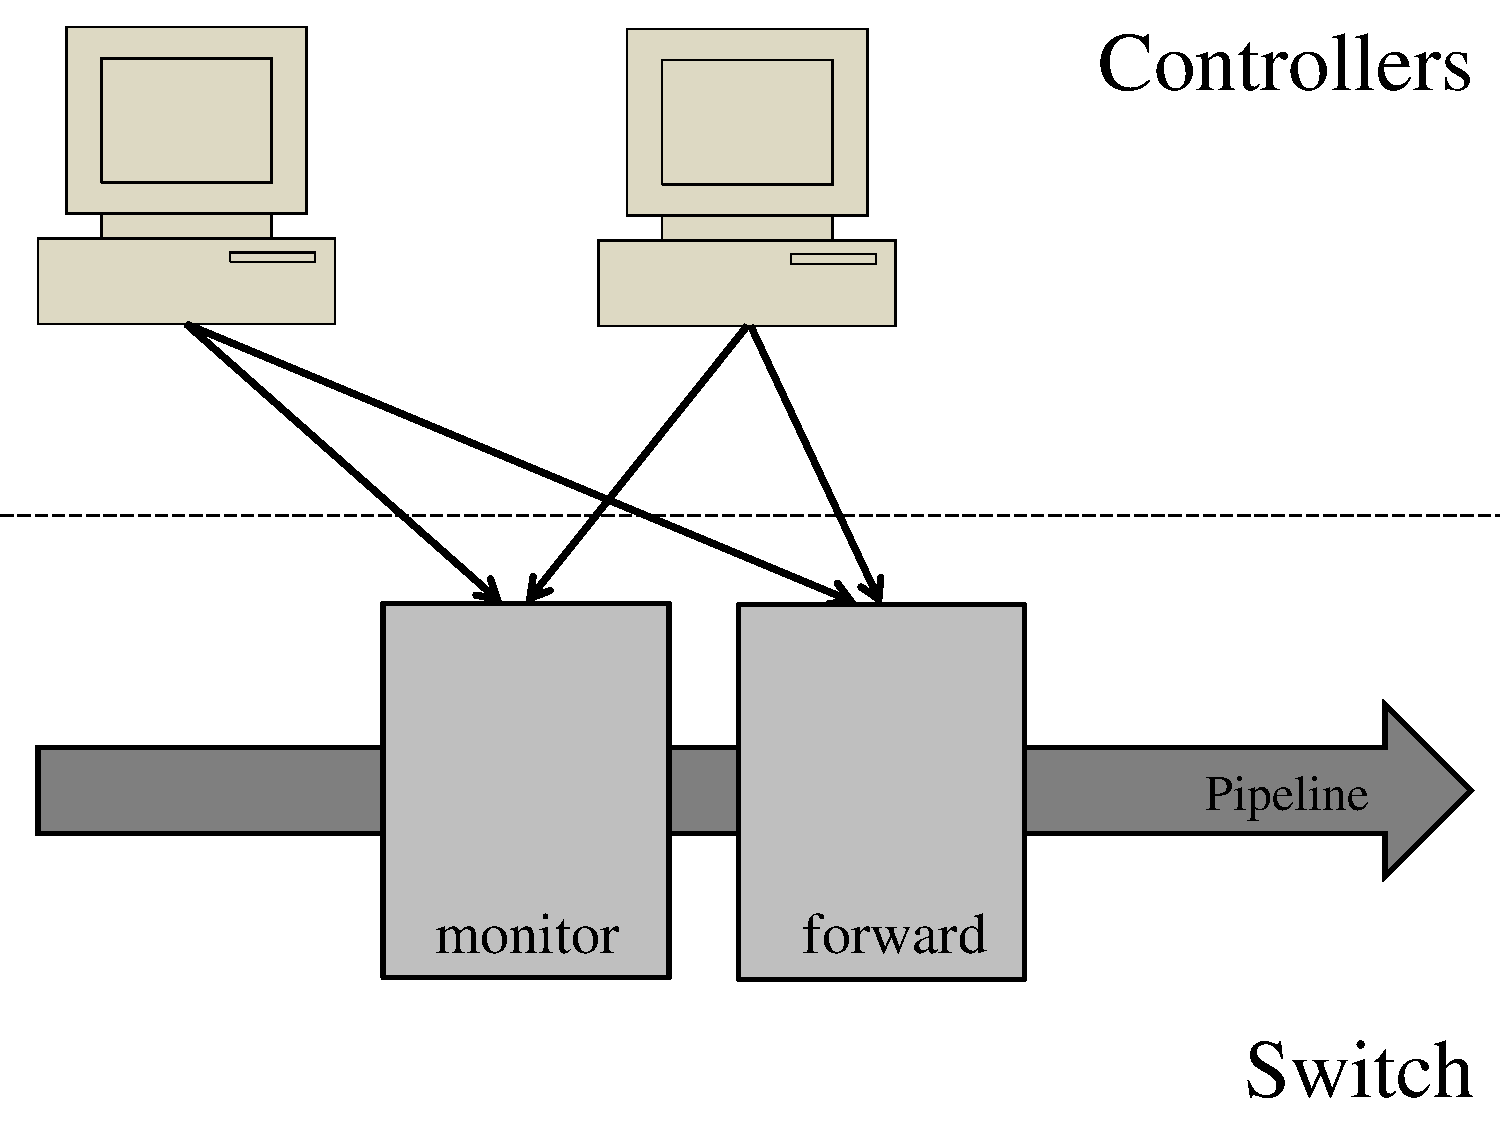
\includegraphics[width=0.8\columnwidth]{composition.pdf}\\
\caption{Composition.}\label{fig:illu}
\end{figure}

\end{comment}

\begin{comment}

\section{Transactions in OpenFlow}\label{sec:sync}

Multi-write and read-modify transactions.

\subsection{Dealing with multiple updates}

TBD - adding the notion of versions and cleanup/GC. probably no good way to solve infinite versions... maybe check literature on shared memory and multiple writes.


\subsection{Improving the scheme with check-overlap}\label{sec:todo}

Till now we considered a model that allows multiple updates to match-action entries. Here we extends the model with actions create-entry and delete-entry that may failed and abort the whole transaction depending on the existence on non-existence of specific entries prior to the action.
%TBD - much less resources. easily solving the infinite versions issue.

Next we show how such actions can be used to implement consensus with much less resources. We use entry id as a property used to reference specific entry.

\section{Applications and ramifications}\label{sec:application}



\section{The Underlying Theory}\label{sec:background}

idea: multi-write consensus, a not well-known result!

In order to solve consensus we suggest to use the atomic multiple entries update capability (which is discussed in OpenFlow standard). A shared memory system that supports atomic write to (enough) multiple locations is known to allow the implementation of consensus objects. For example consider the following implementation utilizing $n^2$ memory locations, $M_{i,j}$, where $i,j\in[n]$, and the suggested values $\{v_i\}_{i\in [n]}$. All locations are initialized to zero.

In order to participate, a server i, writes its suggested value $V_i$ and atomically rewrites row i ($M_{i,*}$) with value "1" and column i ($M_{*,i}$) with value "2". After the atomic write, a server $i$ first reads the diagonal ($M_{j,j}$ for $j\in [n]$), and consider all observed servers as candidate set S.  Then server i reads all candidates intersections (locations $M_{j,k}$ where $j,k\in S$. And computes the winner server id w that was overwritten by all other candidates, i.e. such that $M_{w,k}=2$ for all $k\in S {w}$. The consensus value is $v_w$.
Note that a snapshot could replace the two reading phases.



\section{Basic One-Touch Mechanism}\label{sec:realization}

We address the problem of committing consistent policies to SDN switch concurrently by multiple controllers.
We show that assuming minimalistic control protocol, SDN switch configuration space can be used to implement a consensus object thereby allowing controllers to agree on each next policy update.

\subsection{SDN switch configuration space as shared memory}



Our first observation is that a match-action configuration which is accessed by multiple controllers can be considered as shared memory. Note however that standard memory map and index/offset to a word, while Flow Table entries are not necessarily indexed. However, we assume that each flow entry has some property that allows the operator to specifically reference and update it, for example OpenFlow entry's cookie. In cases where this property value can't be determined by the operator, we can use other variable entry properties to store the index, for example we can represent memory value $v$ in offset $i$ by an match-action entry whose match is $in\_port = i$ and action is "forward port $x$".
%To overcome this we can use the match part of an entry as the index and the action part as the word value.


Going back to the policy update problem, the consensus scheme allow all servers to decide on next policy by using consensus value as policy identifier, and writing the policy in advance. However this scheme doesn't actually apply the policy on incoming packets and it remains to configure the switch according to the next policy once it is decided. Making this scheme fail safe (handling failure of winning server) can be ensured by allowing any server to reconfigure the switch.

\subsection{ One-Touch}

In some scenarios it may be desirable to shorten the policy update time by avoiding the consensus reading and policy configuration step. We define this as the one touch policy update, namely we require each server to contact the switch only once in order to (try and) update the policy, in other words participating in reaching consensus and applying it with one atomic write. Solving this problem also has significance in understanding the strength of the SDN switch computation model.

The main idea of our solution is to adjust the previous policy update scheme in a way that performs consensus validation phase during every packet processing thereby requiring the servers only to make the first phase of the consensus - atomically writing the matrix.
In order to allow the packets to validate the consensus we make the following observation: while servers can be abstracted as memory writers, the packets processed by the switch are the readers. OpenFlow standard define an atomic write transaction as being atomic in relation to the processed packets thereby making packet processing a multiple read transaction but one read location per table is allowed. This means that if each memory location used in the consensus scheme will be stored in different table then each packet will be able to read all of them.

However, reading each memory location is not enough, as the scheme requires to make a validation that involves multiple values. We utilize the metadata field in order to store all read values, in more details, each memory value $M_{i,j}$ is stored in offset i+j*n in the metadata field. Once all values are in the metadata field, we can detect the consensus winner by trying different matches on the metadata. Although we can have one match entry per possible matrix state, this solution requires exponential number of entries. A better way which we describe next requires only $O(n^2)$ entries utilizing n tables.

Our compact validation use additional temp variable, $temp_winner$, to hold the current best consensus candidate. Each of the n validating tables checks different "column" in the matrix and update $temp_winner$ to keep track of the winner so far (after examining a prefix sub set of the columns). The entry t in table k $(0<=k<n)$  matches the case where current winner=t and location $(t,k)$ in the matrix (packet header) equals 1 and location (k,k) is non-zero. After all validating tables are processed, $temp_winner$ stores the id of the winning server which can be used to match on its policy rules (filtering out other policies) or to use the goto table command to jump to a designated policy table of the server.


\section{The Practical Implementation}\label{sec:extension}

\end{comment}

\begin{comment}
\section{Related Work}\label{sec:relwork}

There exists a wide consensus that SDN control planes need to be
distributed~\cite{onos,onix,elasticon}.
Onix~\cite{onix} is one of the earliest proposals, and introduced the
the notion of Network Information Base (NIB), abstracting network state
distribution from control logic, but
requiring mechanisms for the detection and resolution of conflicts.
Also spatially distributed control planes to improve scalability and
latency have been studied intensively
in the literature~\cite{sharon,kandoo,ctrl-place,hotsdn13loc}
proposes an elastic distributed controller architecture.

Operating and updating SDNs efficiently and consistently is already non-trivial
in a setting consisting of a single controller and a single switch.~\cite{sharon}
Reitblatt et al.~\cite{network-update}
introduced the notion of
per-packet consistency and proposed a tagging-based, 2-phase update protocol
which allows a single controller to update network routes.
%, and described the \emph{two-phase update} technique, also used in our algorithms.
Mahajan and Wattenhofer~\cite{roger-hotnets} and Ludwig et al.~\cite{podc15}
considered weaker transient
consistency guarantees, and proposed more efficient network update algorithms
accordingly. Ludwig et al.~~\cite{hotnets14update} studied algorithms for secure
network updates where packets are forced to traverse certain waypoints or
middleboxes. Ghorbani et al.~~\cite{correct-virt} recently argued for the design
of network update algorithms that provide even stronger consistency guarantees.

To the best of our knowledge, the only paper explicitly addressing the consistent
network update problem from a distributed-controllers perspective is STN~\cite{stn}:
STN provides a transactional interface offering all-or-nothing semantics and serializability
(the ``holy grail'' of safety properties), allowing
controllers to install policies in a conflict-free manner; if some controllers fail,
other controllers can take over. STN~\cite{stn} is based on
atomic read-modify-write primitives provided by the switches, but
while the availability of such primitives is postulated, no implementation is
described. Also NetPaxos~\cite{netpaxos} observes the usefulness of
providing synchronization primitives inband, and proposes simple OpenFlow
extensions to implement those.

In this paper, we provide this missing link, and also show that other useful and
more powerful synchronization primitives can be implemented in today's OpenFlow.
Also, the STN protocol~\cite{stn} assumes that the control
plane maintains a certain amount of synchrony which allows controllers
to solve consensus or implement a replicated state machine.
In this paper, we describe an OpenFlow-based consensus protocol that
can be used for this purpose.

Our work is also closely related to the recent work on providing more high-level
abstractions and programming languages for SDNs, such as Frenetic~\cite{frenetic},
also enabling policy composition~\cite{pyretic}. Our work complements these works
on programming abstractions
by initiating the discussion of concurrency objects and abstractions.

The transactional interface we describe in this paper is inspired by the
work on speculative concurrency control using software transactional memory
(STM)~\cite{stm-st95,tm-book}.
%[[PK I think this is enough]]

Our work also contributes to the ongoing discussion of what can be implemented
in-band in OpenFlow~\cite{compute,reclaim}, by focusing on the
relevant problem of synchronization.

\hide{
In terms of distributed computing: TODO PETR: maybe modify a bit the text below
and also write more about multi-writer consensus etc.?

\noindent\textbf{Distributed Computing.}
There is a long tradition of defining correctness of a concurrent system via
an equivalence to a sequential one~\cite{Pap79-serial,Lam79,HW90}.  The notion
of sequentially composable histories is reminiscent of
linearizability~\cite{HW90}, where a history of operations concurrently
applied by a collection of processes is equivalent to a history in which the
operations are in a sequential order, respecting their real-time precedence.
In contrast, our sequentially composable histories impose requirements not
only on high-level invocations and responses, but also on the way the traffic
is processed. We require that the committed policies constitute a
conflict-free sequential history, but, additionally,  we expect that each
\emph{path} witnesses only a prefix of this history, consisting of all
requests that were committed before the path was initiated.
%
The transactional interface exported by the STN abstraction is inspired by the
work on speculative concurrency control using software transactional memory
(STM)~\cite{stm-st95}.
%, thus the  term \emph{software transactional networking}.
Our interface is however intended to model realistic network
management operations, which makes it simpler than recent
dynamic STM models~\cite{dstm}.
%In particular, the sets of rules to be installed by a policy update do not depend on the state of the
%network.

Extending the interface to dynamic policies that adapt their behavior based on
the current network state sounds like a promising research direction.  On the
other hand, our criterion of sequential composability is more complex than
traditional STM correctness properties in that it imposes restrictions not only
on the high-level interface exported to the control plane, but also on the
paths taken by the data plane packets.
Also, we assumed that controllers are subject to failures, which is usually not
assumed by STM implementations.
}

\end{comment}

\section{Conclusion}\label{sec:conclusion}

This paper initiated the study of mechanisms which allow distributed controllers
to synchronize their possibly concurrent actions. We believe that our in-band
approach is natural and attractive as it can avoid the
complexities and limitations of distributed out-of-band agreement protocols.
Moreover, our mechanisms are simple and can be implemented using the \emph{standard OpenFlow}
protocol: they do not require any protocol/hardware extensions as postulated in recent literature~\cite{stn,netpaxos}.
Our work may hence also contribute to the ongoing discussion of what can be implemented
in-band in today's OpenFlow protocol~\cite{reclaim},
as well as to useful high-level concurrency objects and
language abstractions.~\cite{pyretic}
We also plan to release a small library with our synchronization primitives. 
Moreover, we are investigating possible generalizations of our transactional guarantees,
across multiple switches~\cite{stn}, as well as opportunities for more fine-grained
\emph{partial} updates that concern subsets of flow entries, thus improving concurrency. 

%,
%nor on
%nor do we make any assumptions on packet orderings.
%and do not rely on any
%
%.

\begin{comment}
While much progress has been made over the
last years in the development of more intuitive programming
languages for SDNs (e.g., Frenetic, Pyretic, Merlin), the
question of which synchronization abstractions to provide
has received much less attention.
%
In this paper, we describe transactional abstractions that
can be implemented using standard OpenFlow features.
%
Our work complements existing research on the design of
distributed control planes, and also provides some missing links,
e.g., for the transactional approach taken by STN~\cite{stn}.
We also hope that our work can nourish the discussion of
which synchronization objects we can and want to implement
in an SDN.

Even though we believe that we propose efficient and consistent
transactional framework for in-band synchronization, we do not claim
that we offer an exhaustive set of synchronization primitives. Indeed,
one may explore standard OpenFlow features to enable more powerful
primitives. For instance, \emph{cookies}~\cite{openflow} can be used for modifying
flow tables, based on more sophisticated conditions than the default
``exact match''.
Also, the standard pipelining feature allows the switches to maintain multiple flow
tables which can be traversed in arbitrary patterns, defining the sets
of corresponding actions.
Exploring the power of such features is left to future work.
\end{comment}


{
%\begin{footnotesize}
\bibliographystyle{abbrv}
\bibliography{references}  % main.bib is the name of the Bibliography in this case
%\end{footnotesize}
}

\begin{comment}


\clearpage

\onecolumn

\begin{appendix}

\section{The FlowMod Command}

\lstset{% general command to set parameter(s)
	basicstyle=\small, % print whole listing small
	keywordstyle=\color{black}\bfseries, % underlined bold black keywords
	identifierstyle=, % nothing happens
	commentstyle=\color{mygrey}, % white comments
	stringstyle=\ttfamily, % typewriter type for strings
	showstringspaces=false, % no special string spaces
	language=C}
\begin{lstlisting}
struct ofp_flow_mod {
	struct ofp_header header;
	uint64_t cookie; /* Opaque controller-issued identifier. */
	uint64_t cookie_mask; /* Mask used to restrict the cookie bits
		that must match when the command is
		\texttt{ofpfc_{modify}*} or \texttt{ofpfc_{delete}*. A value
		of 0 indicates no restriction. */
	/* Flow actions. */
	uint8_t table_id; /* identifier of the table to put the flow in.
		For OFPFC_DELETE_* commands, OFPTT_ALL
		can also be used to delete matching
		flows from all tables. */
	uint8_t command; /* One of OFPFC_*. */
	uint16_t idle_timeout; /* Idle time before discarding (seconds). */
	uint16_t hard_timeout; /* Max time before discarding (seconds). */
	uint16_t priority; /* Priority level of flow entry. */
	uint32_t buffer_id; /* Buffered packet to apply to, or
		OFP_NO_BUFFER.
		Not meaningful for OFPFC_\dele*. */
	uint32_t out_port; /* For OFPFC_\dele* commands, require
		matching entries to include this as an
		output port. A value of OFPP_ANY
		indicates no restriction. */
	uint32_t out_group; /* For OFPFC_\dele* commands, require
		matching entries to include this as an
		output group. A value of OFPG_ANY
		indicates no restriction. */
	uint16_t flags; /* Bitmap of OFPFF_* flags. */
	uint16_t importance; /* Eviction precedence (optional). */
	struct ofp_match match; /* Fields to match. Variable size. */
	/* The variable size and padded match is always followed by instructions. */
	//struct ofp_instruction_header instructions[0];
		/* Instruction set - 0 or more. The length
		of the instruction set is inferred from
		the length field in the header. */
};
\end{lstlisting}


- Creating an entry with the same match part replaces the existing one.

\section{Bundle Control Message}

%/* Message structure for OFPT_BUNDLE_CTRL. */
\begin{lstlisting}
struct ofp_bundle_ctrl_msg {
	struct ofp_header header;
	uint32_t bundle_id; /* Identify the bundle. */
	uint16_t type; /* OFPBCT_*. */
	uint16_t flags; /* Bitmap of OFPBF_* flags. */
	/* Bundle Property list. */
	struct ofp_bundle_prop_header properties[0]; /* Zero or more properties. */
};
\end{lstlisting}

\begin{lstlisting}
* Adding a message in a bundle is done with. */
struct ofp_bundle_add_msg {
	struct ofp_header header;
	uint32_t bundle_id; /* Identify the bundle. */
	uint16_t pad; /* Align to 64 bits. */
	uint16_t flags; /* Bitmap of OFPBF_* flags. */
	struct ofp_header message; /* Message added to the bundle. */
	/* If there is one property or more, 'message' is followed by:
	* - Exactly (message.length + 7)/8*8 - (message.length) (between 0 and 7)
	* bytes of all-zero bytes */
	/* Bundle Property list. */
	//struct ofp_bundle_prop_header properties[0]; /* Zero or more properties. */
};
\end{lstlisting}

\section{To Be Deleted...}

\begin{algorithm}[h]
    \caption{Policy composition without bundle}
    \label{alg:wobundle}
    \begin{algorithmic}[1]
    \Require policy $P$ (a set of FlowMod entry creation commands), three consecutive flow tables identifiers (per controller) $T_s,T_0,T_1$, active table index $active\in\{0,1\}$.
    %\Ensure installed policy is consistent with previous one
    \State $unactive \gets active + 1 \mod{2}$
    \For {$cmd \in P$}
	    \State $cmd.action\gets Reencode(cmd.action)$
	    \State $cmd.table\_id\gets T_{unactive}$
	    \State send $cmd$
    \EndFor
    \State modify the action of $T_s$ entry to goto $T_{unactive}$
    \State clear table $T_{active}$
    \State $active \gets unactive$
	\Return

    \end{algorithmic}
\end{algorithm}

\begin{algorithm}[h]
    \caption{Update with pipeline}
    \label{alg:pipeline}
    \begin{algorithmic}[1]
    \Require update requirements $U$, array $ARR$.
    \Ensure installed policy is consistent with previous one
			\Return

    \end{algorithmic}
\end{algorithm}


\begin{comment}
\section{Implementing CAS with FlowMod commands}\label{sec:without-groups}
This section describes an implementation without group tables.

Here we describe a second implementation of the Compare\&Set abstraction that is based on entirely on flow entry creations and deletions (FlowMod commands).

The $\checko$ flag enables us to add an entry if no contradicting entry exists and to fail if such do exists. However, the compare stage of \cas requires us to fail if a certain value doesn't exists, i.e. $\cas(x,y)$ failes iff $x \notin T$, where $T$ is the set of match entries defined in a dedicated flow table.
...
...


\begin{algorithm}[H]
    \caption{$\textit{CAS}(old,new)$}
    \label{alg:cas2}
    \begin{algorithmic}[1]
    %\Require  id $i$.
%    \Ensure
			\State $cmds \gets new\ list()$
    		\State $value \gets  old$
    		\State $mask \gets  \texttt{1$\ldots$1}$
    		\State $match \gets (value,mask)$
    		%\State $cookie \gets x\concat self$
    		\State $action \gets 2$
    		\State $flag \gets OFPFF\_\checko$
    		\State $cmd1\gets \emph{FlowMod}(match, op = \add, flag, action) $
    		\State $cmd2\gets \emph{FlowMod}(match, op = \dele) $
    		\State $cmd3\gets \emph{FlowMod}(cookie = old, op = \dele) $
    		\State $cmds.append(cmd1)$
    		\State $cmds.append(cmd2)$
    		\State $cmds.append(cmd3)$
    		\State $range\_matches \gets EncodeRange([0,new-1])\cup EncodeRange([new+1,MAX\_ID])$
    		\For {$r\_match \in range\_matches $}
    		    		\State $cookie \gets new$
    		    		\State $action \gets 1$
    		    		\State $flag \gets 0$
    		    		\State $cmd\gets \emph{FlowMod}(r\_match, \add, flag, cookie, action) $
    		    		\State $cmds.append(cmd)$
    		\EndFor
			\Return $cmds$
    \end{algorithmic}
\end{algorithm}



\section{Implementing CAS with GroupMod commands}\label{sec:with-groups}
Similarly, we use a deletion of group $x$ and a creation of group $y$ (with GroupMod commands) as an
abstraction to performing a $CAS(x,y)$ operation to a special $16$bit register (we abstract only one register). The $16$ bit limit is resulted by th $16$bit group id size.
%The group id of the added group represents the added number.
Note that trying to delete a group that doesn't exist (or trying to create a group with id that already exists) fails, thereby preventing adding the new value $y$ if $x$ hasn't existed before. Note that the two action should be performed inside the same bundle in order to ensure the atomic nature ot the abstraction.

\begin{algorithm}[H]
    \caption{$\textit{group-CAS}(old,new)$}
    \label{alg:gcas}
    \begin{algorithmic}[1]
    %\Require  id $i$.
%    \Ensure

    		\State $op \gets \texttt{OFPGC\_\dele}$
    		\State $group\_id \gets old$
    		\State $cmd1\gets GroupMod(op, group\_id) $
    		
    		\State $op \gets \texttt{OFPGC\_\add}$
    		\State $type \gets \texttt{OFPGT\_INDIRECT}$
    		\State $group\_id \gets new$
    		\State $buckets \gets [dummy\_backet]$
    		\State $cmd2\gets GroupMod(op, type, group\_id, buckets) $
			\Return $cmd1,cmd2$
    \end{algorithmic}
\end{algorithm}

\begin{comment}
\section{Backup Stuff}

using the bundling feature to implement \emph{multi-write} or, more
widely, \emph{multi-modify} transactions. .
, using a single OpenFlow switch that accepts
bundle control messages.

We first show that they can be used to replace the read-modify-write
primitives voluntarily assumed in the recent implementation of a
recent proposal for a consistent composition system for forwarding policies~\cite{stn}.
We then use these transactions directly to implement a lightweight
forwarding policy composition system that requires no additional
synchronization on the control plane.
We then explore how more general classes of policies can be composed
\emph{on-the-switch}.

TODO: write vision and contribution in full detail, as an overview


using the bundling feature to implement \emph{multi-write} or, more
widely, \emph{multi-modify} transactions. .
, using a single OpenFlow switch that accepts
bundle control messages.

We first show that they can be used to replace the read-modify-write
primitives voluntarily assumed in the recent implementation of a
recent proposal for a consistent composition system for forwarding policies~\cite{stn}.
We then use these transactions directly to implement a lightweight
forwarding policy composition system that requires no additional
synchronization on the control plane.
We then explore how more general classes of policies can be composed
\emph{on-the-switch}.

TODO: write vision and contribution in full detail, as an overview

we can do more than container:

we introduce container: it's not compare+set, ... its something new!
new object, is stronger than compare and set because bundle!


\end{appendix}

\end{comment}

\end{document}
